%%%%%%%%%%%%%%%%%%%%%%%%%%%%%%%%%%%%%
% Check out the accompanying book, Even Better Books with LaTeX the Agile Way in 2023, for a discussion of the template and step-by-step instructions. https://amzn.to/3HqwgXM https://leanpub.com/eBBwLtAW/
% The template was originally created by Clemens Lode, LODE Publishing (www.lode.de), on 1/1/2023. Feel free to use this template for your book project!
% I would be happy if you included a short mention in your book in order to help others to create their own books, too ("Book template based on \textit{Even Better Books with LaTeX the Agile Way in 2023} by Clemens Lode").
% Contact me at mail@lode.de if you need help with the template or are interested in our editing and publishing services.
% And don't forget to follow us on Instagram! https://www.instagram.com/lodepublishing/ https://www.instagram.com/betterbookswithlatex/
%%%%%%%%%%%%%%%%%%%%%%%%%%%%%%%%%%%%%

% To create an EPUB file, select pdfLaTeX in the Menu in the top-left and choose the conversion method in the /latexmkrc file.

% Select document class scrbook to be in the two-page mode and accommodate for the binding of a printed book.
% The bibliography receives an entry in the table of contents but no number.
\documentclass[
    pagesize=auto,
    bibliography=totocnumbered,
    cleardoublepage=empty
    ]{scrbook}

%%%%%%%%%%%%%%%%%%%%%%%%%%%%%%%%%%%%%
% Check out the accompanying book, Even Better Books with LaTeX the Agile Way in 2023, for a discussion of the template and step-by-step instructions. https://amzn.to/3HqwgXM https://leanpub.com/eBBwLtAW/
% The template was originally created by Clemens Lode, LODE Publishing (www.lode.de), on 1/1/2023. Feel free to use this template for your book project!
% I would be happy if you included a short mention in your book in order to help others to create their own books, too ("Book template based on \textit{Even Better Books with LaTeX the Agile Way in 2023} by Clemens Lode").
% Contact me at mail@lode.de if you need help with the template or are interested in our editing and publishing services.
% And don't forget to follow us on Instagram! https://www.instagram.com/lodepublishing/ https://www.instagram.com/betterbookswithlatex/
%%%%%%%%%%%%%%%%%%%%%%%%%%%%%%%%%%%%%

% Replace "The Title" with your book title.
\newcommand{\mytitle}{The Title}

% Replace "The subtitle" with your book's subtitle.
\newcommand{\mysubtitle}{The subtitle}

% Replace "Publishing Company" with the name of the publishing company it is published.
\newcommand{\mypublishingcompany}{Daniel Díaz Quílez}

% Replace "Location of the Publishing Company (city)" with the location (e.g., the city) of the publishing company.
\newcommand{\mypublishingcompanylocation}{Helsinki, Finlandia}

\newcommand{\mypublishingcompanyurl}{\url{https://www.lode.de}}


% Upload a low-resolution jpg (e-book) and a high-resolution (pdf/print) png version of your front cover into the "images" folder. If you need help with creating a cover, email us at mail@lode.de to talk about what you need, and we will do our best to help you.
\newcommand{\coverImage}{images/cover.jpg}
\newcommand{\hiresCoverImage}{images/cover.png}


% Replace "Your email address" with your email address.
% Replace "Edition" with the edition number.
% Replace the ISBNs with your ISBNs.
% Replace "Your editor's name" with your editor's name.
% Replace "Your designer's name" with your book cover designer's name.
% Replace "Your image sources" with the sources of your images (including icons) and relevant license information.
% Replace "Your newsletter email" with your newsletter email.
% Replace "Your newsletter URL" with your website's newsletter URL.


\newcommand{\mypublishingcompanyemail}{Your email address}
\newcommand{\editionNumber}{First}

% Buy ISBNs or use the ISBNs generated by Amazon and list them  here.
\newcommand{\ebookISBN}{123-4-567890-12-3}
\newcommand{\softcoverISBN}{123-4-567890-12-4}
\newcommand{\hardcoverISBN}{123-4-567890-12-5}

\newcommand{\editorName}{Daniel Díaz Quílez}
\newcommand{\designerName}{Daniel Díaz Quílez}
\newcommand{\typesetterName}{Daniel Díaz Quílez}
\newcommand{\imageSources}{Daniel Díaz Quílez}

\newcommand{\newsletterMail}{Your newsletter email}
\newcommand{\newsletterURL}{Your newsletter URL}

% If you want to subscribe to this book's newsletter, write an email to newsletter@lode.de or follow us on Instagram.com/lodepublishing or Instagram/betterbookswithlatex

\newcommand{\yourName}{Your name}

% Replace city, country, and date with the place and country where you (or your company) are located and the date when the preface was finished (it does not have to be the release date of the book).

\newcommand{\yourCity}{Your city}
\newcommand{\yourCountry}{Your country}
\newcommand{\prefaceDate}{\today}

\newif\ifuseAuthorImage
% Uncomment and upload author images
%\useAuthorImagetrue

\ifuseAuthorImage
    \newcommand{\authorImage}{images/author.jpg}
    \newcommand{\authorImageHiRes}{images/author.png}
\fi


% Uncomment \seriestrue if your book is part of a series.
\newif\ifseries
%\seriestrue

\ifseries
% Replace "Title of Book Series" with the title of the book series.
% Replace "Title of Part One" with the title of part one.
% Replace "Title of Part Two" with the title of part two.
% Replace "Title of Part Three" with the title of part three, or remove the line if there is no part three.
% Replace "Title of Part Four" with the title of part four, or remove the line if there is no part four.

\newcommand{\partOneTitle}{Title of Part One}
\newcommand{\partTwoTitle}{Title of Part Two}
\newcommand{\partThreeTitle}{Title of Part Three}
\newcommand{\partFourTitle}{Title of Part Four}

\newcommand{\titleOfTheBookSeries}{Title of the Book Series}

\newif\firstBookOfSeries
\firstBookOfSeries

\ifFirstBookOfSeries
\else
\newcommand{\partPreviousPart}{Number of the previous part in the book series}
\newcommand{\titlePreviousPart}{Title of the previous part in the book series}

\newcommand{\previousCoverImage}{images/previous_part_of_the_series_Cover.jpg}
\newcommand{\previousCoverImageHiRes}{images/previous_part_of_the_series_Cover_hires.png}

\fi


% If you want a different size than 6"x9", change the lib/bookformat.tex file accordingly.

\newif\ifhardcover
% Uncomment for selecting hardcover.
%\hardcovertrue

\title{\mytitle}

% Load additional LaTeX libraries.
%%%%%%%%%%%%%%%%%%%%%%%%%%%%%%%%%%%%% 
% Check out the accompanying book, Even Better Books with LaTeX the Agile Way in 2023, for a discussion of the template and step-by-step instructions. https://amzn.to/3HqwgXM https://leanpub.com/eBBwLtAW/
% The template was originally created by Clemens Lode, LODE Publishing (www.lode.de), on 1/1/2023. Feel free to use this template for your book project! 
% I would be happy if you included a short mention in your book in order to help others to create their own books, too ("Book template based on \textit{Even Better Books with LaTeX the Agile Way in 2023} by Clemens Lode").
% Contact me at mail@lode.de if you need help with the template or are interested in our editing and publishing services.
% And don't forget to follow us on Instagram! https://www.instagram.com/lodepublishing/ https://www.instagram.com/betterbookswithlatex/
%%%%%%%%%%%%%%%%%%%%%%%%%%%%%%%%%%%%%



% This configures the PDF/EPUB output.
%%%%%%%%%%%%%%%%%%%%%%%%%%%%%%%%%%%%% 
% Check out the accompanying book, Even Better Books with LaTeX the Agile Way in 2023, for a discussion of the template and step-by-step instructions. https://amzn.to/3HqwgXM https://leanpub.com/eBBwLtAW/
% The template was originally created by Clemens Lode, LODE Publishing (www.lode.de), on 1/1/2023. Feel free to use this template for your book project! 
% I would be happy if you included a short mention in your book in order to help others to create their own books, too ("Book template based on \textit{Even Better Books with LaTeX the Agile Way in 2023} by Clemens Lode").
% Contact me at mail@lode.de if you need help with the template or are interested in our editing and publishing services.
% And don't forget to follow us on Instagram! https://www.instagram.com/lodepublishing/ https://www.instagram.com/betterbookswithlatex/
%%%%%%%%%%%%%%%%%%%%%%%%%%%%%%%%%%%%%

% This command enables checking if XeLaTeX is used.
\usepackage{ifxetex}

\ifxetex
    % For the PDF output, load the following additional packages.
    
    % This adjusts figures to fit into the width of a page.
    \usepackage{adjustbox}
    
    % Use this for fancy lines at the beginning of chapters and the end of sections.
    \usepackage{psvectorian} 

\else
    % Ignore adjustbox commands (HTML files do not have a width).
    \newcommand{\adjustbox}[2][]{#1}

    % Ignore psvectorian lines.
    \newcommand{\psvectorian}[2][]{}
\fi

% Translate newpage and hrule commands.
\ifx\HCode\undefined
    \newcommand{\nextpage}[1][]{}
\else
    \newcommand{\nextpage}[1][]{\HCode{<mbp:pagebreak />}}
    \renewcommand{\hrule}{\HCode{<hr style="clear: both" />}}
\fi

% Sets up support for multiple languages.
%%%%%%%%%%%%%%%%%%%%%%%%%%%%%%%%%%%%%
% Check out the accompanying book, Even Better Books with LaTeX the Agile Way in 2023, for a discussion of the template and step-by-step instructions. https://amzn.to/3HqwgXM https://leanpub.com/eBBwLtAW/
% The template was originally created by Clemens Lode, LODE Publishing (www.lode.de), on 1/1/2023. Feel free to use this template for your book project!
% I would be happy if you included a short mention in your book in order to help others to create their own books, too ("Book template based on \textit{Even Better Books with LaTeX the Agile Way in 2023} by Clemens Lode").
% Contact me at mail@lode.de if you need help with the template or are interested in our editing and publishing services.
% And don't forget to follow us on Instagram! https://www.instagram.com/lodepublishing/ https://www.instagram.com/betterbookswithlatex/
%%%%%%%%%%%%%%%%%%%%%%%%%%%%%%%%%%%%%

% Activate American language (and \babelEN).
% \usepackage[american]{babel}

% Activate Spanish language (and \babelES).
\usepackage[spanish]{babel}

% Activate German language (and \babelDE).
%\usepackage[ngerman]{babel}

% Fix PDF creation.
\ifxetex
	\let\pdfstrcmp\strcmp
\fi
% Set up macros to support multiple languages:
\newcommand{\babelES}[1]{\ifnum\pdfstrcmp{\languagename}{spanish}=0 {#1}\fi}
\newcommand{\babelDE}[1]{\ifnum\pdfstrcmp{\languagename}{ngerman}=0 {#1}\fi}
\newcommand{\babelEN}[1]{\ifnum\pdfstrcmp{\languagename}{american}=0 {#1}\fi}

\addto\captionsspanish{%
  \renewcommand{\contentsname}{Índice}%
}


% Loads packages to be able to configure hyphenation.
%%%%%%%%%%%%%%%%%%%%%%%%%%%%%%%%%%%%% 
% Check out the accompanying book, Even Better Books with LaTeX the Agile Way in 2023, for a discussion of the template and step-by-step instructions. https://amzn.to/3HqwgXM https://leanpub.com/eBBwLtAW/
% The template was originally created by Clemens Lode, LODE Publishing (www.lode.de), on 1/1/2023. Feel free to use this template for your book project! 
% I would be happy if you included a short mention in your book in order to help others to create their own books, too ("Book template based on \textit{Even Better Books with LaTeX the Agile Way in 2023} by Clemens Lode").
% Contact me at mail@lode.de if you need help with the template or are interested in our editing and publishing services.
% And don't forget to follow us on Instagram! https://www.instagram.com/lodepublishing/ https://www.instagram.com/betterbookswithlatex/
%%%%%%%%%%%%%%%%%%%%%%%%%%%%%%%%%%%%%

% Use fontenc to properly hyphenate accented languages.
\usepackage[T1]{fontenc}

% Add a list of words to enforce a certain hyphenation for them.
\usepackage{hyphenat}
\hyphenation{}



% In this package, we define the dimensions of the printed book.
%%%%%%%%%%%%%%%%%%%%%%%%%%%%%%%%%%%%%
% Check out the accompanying book, Even Better Books with LaTeX the Agile Way in 2023, for a discussion of the template and step-by-step instructions. https://amzn.to/3HqwgXM https://leanpub.com/eBBwLtAW/
% The template was originally created by Clemens Lode, LODE Publishing (www.lode.de), on 1/1/2023. Feel free to use this template for your book project!
% I would be happy if you included a short mention in your book in order to help others to create their own books, too ("Book template based on \textit{Even Better Books with LaTeX the Agile Way in 2023} by Clemens Lode").
% Contact me at mail@lode.de if you need help with the template or are interested in our editing and publishing services.
% And don't forget to follow us on Instagram! https://www.instagram.com/lodepublishing/ https://www.instagram.com/betterbookswithlatex/
%%%%%%%%%%%%%%%%%%%%%%%%%%%%%%%%%%%%%

%%%%%%%%%%%%%%%%%
% Configure bleed.
%%%%%%%%%%%%%%%%%

% If your book includes images that extend beyond the usual margins, set bleed to 0.125in and activate the corresponding option in Amazon KDP.

\newcommand{\margintop}{1.65cm}
\newcommand{\marginbottom}{2.0cm}
\newcommand{\marginoutside}{1.5cm}

%%%%%%%%%%%%%%%%%
% The inner margins depend on the number of pages of your book.
%%%%%%%%%%%%%%%%%

% Note that books printed by Amazon have an upper limit of number of pages. This limits depends on your book's dimensions, whether it is a paperback or hardcover format, and whether it is printed in black and white or in color.
% See https://kdp.amazon.com/en_US/help/topic/GVBQ3CMEQW3W2VL6

% Select the margin for 24 - 150 pages by default.
\newcommand{\margininside}{1.5cm}

%%%%%%%%%%%%%%%%%
% Hardcover / Softcover Formats. Selecting one of these ensures that you can use the same PDF for hardcover and softcover books on Amazon.
%%%%%%%%%%%%%%%%%

% Select 5x8 by default.
\newcommand{\bookwidth}{5in}
\newcommand{\bookheight}{8in}

%%%%%%%%%%%%%%%%%
% Hardcover-only formats. Selecting one of these requires you to create a separate PDF for a softcover version.
%%%%%%%%%%%%%%%%%

%\newcommand{\bookwidth}{8.25in}\newcommand{\bookheight}{11in}

%%%%%%%%%%%%%%%%%
% Softcover-only formats. Selecting one of these requires you to create a separate PDF for a hardcover version.
%%%%%%%%%%%%%%%%%

%\newcommand{\bookwidth}{5in}\newcommand{\bookheight}{8in}
%\newcommand{\bookwidth}{5.25in}\newcommand{\bookheight}{8in}
%\newcommand{\bookwidth}{5.06in}\newcommand{\bookheight}{7.81in}
%\newcommand{\bookwidth}{6.69in}\newcommand{\bookheight}{9.61in}
%\newcommand{\bookwidth}{7.44in}\newcommand{\bookheight}{9.69in}
%\newcommand{\bookwidth}{7.5in}\newcommand{\bookheight}{9.25in}
%\newcommand{\bookwidth}{8in}\newcommand{\bookheight}{10in}
%\newcommand{\bookwidth}{8.5in}\newcommand{\bookheight}{11in}

%%%%%%%%%%%%%%%%%
% And now we are putting everything together to set the dimensions of the book.
%%%%%%%%%%%%%%%%%

\usepackage[
    paperwidth=\bookwidth,
    paperheight=\bookheight,
    inner=\margininside,
    outer=\marginoutside,
    top=\margintop,
    bottom=\marginbottom,
    includehead,
    includefoot,
    headheight=0pt,
    bindingoffset=6mm
]{geometry}


% This package defines all the box commands.
%%%%%%%%%%%%%%%%%%%%%%%%%%%%%%%%%%%%% 
% Check out the accompanying book, Even Better Books with LaTeX the Agile Way in 2023, for a discussion of the template and step-by-step instructions. https://amzn.to/3HqwgXM https://leanpub.com/eBBwLtAW/
% The template was originally created by Clemens Lode, LODE Publishing (www.lode.de), on 1/1/2023. Feel free to use this template for your book project! 
% I would be happy if you included a short mention in your book in order to help others to create their own books, too ("Book template based on \textit{Even Better Books with LaTeX the Agile Way in 2023} by Clemens Lode").
% Contact me at mail@lode.de if you need help with the template or are interested in our editing and publishing services.
% And don't forget to follow us on Instagram! https://www.instagram.com/lodepublishing/ https://www.instagram.com/betterbookswithlatex/
%%%%%%%%%%%%%%%%%%%%%%%%%%%%%%%%%%%%%

% Replace the "Did you know?", "Read more in...", box titles, and icons if necessary.

% Configuring the commands for the PDF output...
\ifx\HCode\undefined 

    % If you want to add a picture to the top right corner of a box, uncomment the line and upload the picture.

    \usepackage[many]{tcolorbox}
    
    \newtcolorbox{problem}[1][]{colframe = black!30,colback  = black!4,coltitle = black!20!black,title=\babelDE{\textbf{Frage}}\babelEN{\textbf{Question}}
    %\hfill\smash{\raisebox{-11pt}{\includegraphics[height=1cm]{images/speech-bubble-cloud-with-question-mark.png}}}
    , #1,}
    
    \newtcolorbox{idea}[1][]{colframe = black!30,colback  = black!5,coltitle = black!30!black,title=\babelDE{\textbf{Idee}}\babelEN{\textbf{Idea}}
    %\hfill\smash{\raisebox{-11pt}{\includegraphics[height=1cm]{images/lightbulb-idea}}}
    , #1,}

    \newtcolorbox{example}[1][]{colframe = black!20,colback  = black!0,coltitle = black!20!black,title=\babelDE{\textbf{Beispiel}}\babelEN{\textbf{Example}}
    %\hfill\smash{\raisebox{-11pt}{\includegraphics[height=1cm]{images/book-and-test-tube-with-supporter}}}
    , #1,}

    
    \newtcolorbox{biography}[2][]{colframe = black!30,colback  = black!5,coltitle = black!30!black,title=\babelDE{Biographie -- }\babelEN{Biography---}\textbf{#2}
    %\hfill\smash{\raisebox{-11pt}{\includegraphics[height=1cm]{images/identity-card}}}
    , #1,}
    
% ... and for the HTML output.
\else
	
    \newenvironment{problem}[1][]{\bfseries\HCode{<b>}}{\HCode{</b>}\par}
    
    \newenvironment{idea}[1][]{\bfseries\HCode{<b>}}{\HCode{</b>}\par}
	
    \newenvironment{example}[1][]{\hrule\par \textbf{\babelDE{Beispiel}\babelEN{Example}}\par}{\hrule\par}
    
    \newenvironment{biography}[2][]{\hrule\par\textbf{\babelDE{Biographie}\babelEN{Biography}} \emdash \textbf{#2}\par}{\hrule\par}

\fi



% Print out listings as-is (ignoring any special characters).
\usepackage{listings}




\ifx\HCode\undefined 

% This code loads the \leftbar command for the definition environment.
    \usepackage{framed}
    \newenvironment{definition}[2][]{\begin{leftbar}\textbf{\textsc{#2}}\ ·\ #1}{\end{leftbar}\vspace{-\baselineskip}}


% Create a new environment "myquotation" that indents a whole paragraph to show that it is not part of the normally flowing text.
    \renewcommand{\indent}{\begin{picture}(0,0)\put(10,-5){\makebox(0,0){\scalebox{6}{\textcolor{lightgray}{``}}}}\end{picture}\hspace*{1.0cm}\hangindent=1.15cm}
    \newenvironment{myquotation}{\indent}{}

\else
    \newenvironment{definition}[2][]{\textbf{\textsc{#2}}\ ·\ #1}

% For the HTML output for the e-book, the indentation is defined in the style.css.
    \newenvironment{myquotation}
    {\begin{quotation}}{\end{quotation}}

    
\fi



% Uncomment this command for more error and warning messages.
%%%%%%%%%%%%%%%%%%%%%%%%%%%%%%%%%%%%%% 
% Check out the accompanying book, Even Better Books with LaTeX the Agile Way in 2023, for a discussion of the template and step-by-step instructions. https://amzn.to/3HqwgXM https://leanpub.com/eBBwLtAW/
% The template was originally created by Clemens Lode, LODE Publishing (www.lode.de), on 1/1/2023. Feel free to use this template for your book project! 
% I would be happy if you included a short mention in your book in order to help others to create their own books, too ("Book template based on \textit{Even Better Books with LaTeX the Agile Way in 2023} by Clemens Lode").
% Contact me at mail@lode.de if you need help with the template or are interested in our editing and publishing services.
% And don't forget to follow us on Instagram! https://www.instagram.com/lodepublishing/ https://www.instagram.com/betterbookswithlatex/
%%%%%%%%%%%%%%%%%%%%%%%%%%%%%%%%%%%%%


% Activate warnings about outdated/invalid packages.
\RequirePackage[l2tabu, orthodox]{nag}

% Configure LaTeX to provide full error messages.
\errorcontextlines 10000

% Loading this package sets up a balanced multicol environment that can end mid-page (needs to be loaded before fonts because of imakeidx package).
%%%%%%%%%%%%%%%%%%%%%%%%%%%%%%%%%%%%% 
% Check out the accompanying book, Even Better Books with LaTeX the Agile Way in 2023, for a discussion of the template and step-by-step instructions. https://amzn.to/3HqwgXM https://leanpub.com/eBBwLtAW/
% The template was originally created by Clemens Lode, LODE Publishing (www.lode.de), on 1/1/2023. Feel free to use this template for your book project! 
% I would be happy if you included a short mention in your book in order to help others to create their own books, too ("Book template based on \textit{Even Better Books with LaTeX the Agile Way in 2023} by Clemens Lode").
% Contact me at mail@lode.de if you need help with the template or are interested in our editing and publishing services.
% And don't forget to follow us on Instagram! https://www.instagram.com/lodepublishing/ https://www.instagram.com/betterbookswithlatex/
%%%%%%%%%%%%%%%%%%%%%%%%%%%%%%%%%%%%%

% Balance the contents of two columns (as opposed to filling first the left column and then the right). This is used for the glossary.
% See https://tex.stackexchange.com/questions/241094/multicol-column-balancing-only-after-a-minimum-number-of-lines

\ifxetex
\usepackage[balancingshow]{multicol}
\usepackage{regexpatch}

\newcounter{multicolminlines}
\setcounter{multicolminlines}{1}

\makeatletter
\xpatchcmd\balance@columns
   {\ifnum\dimen@<\topskip
     \mult@info\@ne
       {Start value
          \the\dimen@  \space ->
          \the\topskip \space (corrected)}%
     \dimen@\topskip
   \fi}
   {\skip@\c@multicolminlines\baselineskip
   \advance\skip@-\baselineskip
   \advance\skip@\topskip
   \ifnum\dimen@<\skip@
     \mult@info\@ne
       {Start value
          \the\dimen@  \space ->
          \the\skip@ \space (corrected)}%
     \dimen@\skip@
   \fi
   }
   {\typeout{Success!}}{\patchFAILED}
\makeatother
\else

    \newenvironment{multicols}[2][]{}{}

\fi


% Loads the bibliography support and the bibliography files.
%%%%%%%%%%%%%%%%%%%%%%%%%%%%%%%%%%%%%
% Check out the accompanying book, Even Better Books with LaTeX the Agile Way in 2023, for a discussion of the template and step-by-step instructions. https://amzn.to/3HqwgXM https://leanpub.com/eBBwLtAW/
% The template was originally created by Clemens Lode, LODE Publishing (www.lode.de), on 1/1/2023. Feel free to use this template for your book project!
% I would be happy if you included a short mention in your book in order to help others to create their own books, too ("Book template based on \textit{Even Better Books with LaTeX the Agile Way in 2023} by Clemens Lode").
% Contact me at mail@lode.de if you need help with the template or are interested in our editing and publishing services.
% And don't forget to follow us on Instagram! https://www.instagram.com/lodepublishing/ https://www.instagram.com/betterbookswithlatex/
%%%%%%%%%%%%%%%%%%%%%%%%%%%%%%%%%%%%%

%%%%%%%%%%%%%%%%%
% Set up the bibliography.
%%%%%%%%%%%%%%%%%


\ifxetex
% See https://www.ctan.org/pkg/biblatex for documentation.
	\usepackage[indexing=cite,style=authoryear,sortlocale=de_DE,natbib=true]{biblatex}
\else
	\usepackage{natbib}
	\usepackage{usebib}

	% \citetitle does not work with natbib / pdfLaTeX -> translate into \usebibentry
	\newcommand{\citetitle}[2][]{\textit{\usebibentry{#2}{title}}}
\fi

% Load the corresponding bibliography files.
\ifxetex
	\babelEN{\addbibresource{chapters/bibliography/english.bib}}
\else
    \babelEN{\bibinput{chapters/bibliography/english}}
\fi


% Add a command to allow a preface for the bibliography (optional).
\newcommand{\bibpreface}[1]{\patchcmd{\thebibliography}{\list}{#1\list}{}{}}



% Use csquotes to correctly typeset quoted text according to the selected language.
\usepackage{csquotes}


% Write the name of a referenced section or chapter label with \nameref{label}.
\usepackage{nameref}
\newcommand{\reference}[2][]{see \nameref{#2}, Chapter~\ref{#2}}


% This package loads and configures the fonts we use.
%%%%%%%%%%%%%%%%%%%%%%%%%%%%%%%%%%%%%
% Check out the accompanying book, Even Better Books with LaTeX the Agile Way in 2023, for a discussion of the template and step-by-step instructions. https://amzn.to/3HqwgXM https://leanpub.com/eBBwLtAW/
% The template was originally created by Clemens Lode, LODE Publishing (www.lode.de), on 1/1/2023. Feel free to use this template for your book project!
% I would be happy if you included a short mention in your book in order to help others to create their own books, too ("Book template based on \textit{Even Better Books with LaTeX the Agile Way in 2023} by Clemens Lode").
% Contact me at mail@lode.de if you need help with the template or are interested in our editing and publishing services.
% And don't forget to follow us on Instagram! https://www.instagram.com/lodepublishing/ https://www.instagram.com/betterbookswithlatex/
%%%%%%%%%%%%%%%%%%%%%%%%%%%%%%%%%%%%%


% Set font size of captions to small.
\ifxetex
    \usepackage[labelfont=bf]{caption}
    \captionsetup{font=small}
\fi

% Use this shorter command for textemdash.
\newcommand{\emdash}[1][]{\textemdash}

% Set bibliography to footnote size.
\renewcommand{\bibfont}{\footnotesize}
% You can use ``same'' (same font as your document's), ``sf'', ``tt''  or ``rm'' for monospaced font. Also see https://www.ctan.org/pkg/url
\usepackage{url}
\urlstyle{same}

%-------------------------------------------
% Create hyperlinks within PDF files but do not mark them as links.
\ifxetex
    \usepackage{hyperref}[2011/02/05]
    \hypersetup{hidelinks}
\fi

% The following commands improve the font face for the PDF output (font tweaks are not available for e-books).
\ifxetex
% Prevent splitting footnotes over several pages. See https://texfaq.org/FAQ-splitfoot
    \interfootnotelinepenalty=10000

% Set the footnote font size to very small.
    \renewcommand{\footnotesize}{\scriptsize}


% Set the font size of the index to very small.
    \usepackage{imakeidx}
    \indexsetup{othercode=\footnotesize}

% Use this command if you prefer more spaces between words rather than more hyphenations at the end of a line.
    \sloppy

% To slightly tweak font spacing for aesthetics, use these commands.
    \usepackage{microtype}
    \usepackage{lmodern}

% Use Linux Libertine font. For other fonts, check out http://www.tug.dk/FontCatalogue/
    \usepackage{libertine}
\fi

% Required packages to avoid warnings when switching to setting the language to Spanish
\usepackage[T1]{fontenc}
\usepackage{lmodern}
\usepackage[scale=0.9]{tgheros}


% This initializes the TikZ system.
%%%%%%%%%%%%%%%%%%%%%%%%%%%%%%%%%%%%% 
% Check out the accompanying book, Even Better Books with LaTeX the Agile Way in 2023, for a discussion of the template and step-by-step instructions. https://amzn.to/3HqwgXM https://leanpub.com/eBBwLtAW/
% The template was originally created by Clemens Lode, LODE Publishing (www.lode.de), on 1/1/2023. Feel free to use this template for your book project! 
% I would be happy if you included a short mention in your book in order to help others to create their own books, too ("Book template based on \textit{Even Better Books with LaTeX the Agile Way in 2023} by Clemens Lode").
% Contact me at mail@lode.de if you need help with the template or are interested in our editing and publishing services.
% And don't forget to follow us on Instagram! https://www.instagram.com/lodepublishing/ https://www.instagram.com/betterbookswithlatex/
%%%%%%%%%%%%%%%%%%%%%%%%%%%%%%%%%%%%%

% Tikz configuration. For details, see the main manual at  http://www.texample.net/media/pgf/builds/pgfmanualCVS2012-11-04.pdf

\usepackage{tikz}
% The pgfplots package is incompatible with tikzexternalize.
%\usepackage{pgfplots}

% Enable the usage of floats (like figures or tables) which can be placed exactly where they are defined.
\usepackage{float}

% Load various tikz libraries; you might need only some of them (or additional ones).
\usetikzlibrary{matrix,calc,positioning,shapes.arrows,shapes.symbols,decorations.pathreplacing,patterns,shapes,backgrounds,lindenmayersystems,shadings,intersections}

% Define styles of various tikz elements.
\tikzstyle{every node}=[font=\small,node distance=40pt and 50pt,thick]
\tikzstyle{textbox} = [rounded corners, text width=60pt, minimum height=50pt,text centered,draw=black]
\tikzstyle{arrow} = [thick,->,>=latex]
\tikzstyle{largearrow} = [thick,right of=book,draw,single arrow head indent=0ex,single arrow, rotate=90,node distance=130pt,text width=160pt,text centered]
\tikzstyle{block} = [rectangle,textbox]
\tikzstyle{textarr} = [rectangle,align=center,fill=white]
\tikzstyle{print} = [draw,tape,tape bend top=none,tape bend height=15pt,textbox]
\tikzstyle{wave} = [draw,tape,tape bend height=10pt,text width=60pt, minimum height=50pt,text centered,draw=black]


% This package defines the blankpage command and configures page numbering.
%%%%%%%%%%%%%%%%%%%%%%%%%%%%%%%%%%%%%
% Check out the accompanying book, Even Better Books with LaTeX the Agile Way in 2023, for a discussion of the template and step-by-step instructions. https://amzn.to/3HqwgXM https://leanpub.com/eBBwLtAW/
% The template was originally created by Clemens Lode, LODE Publishing (www.lode.de), on 1/1/2023. Feel free to use this template for your book project!
% I would be happy if you included a short mention in your book in order to help others to create their own books, too ("Book template based on \textit{Even Better Books with LaTeX the Agile Way in 2023} by Clemens Lode").
% Contact me at mail@lode.de if you need help with the template or are interested in our editing and publishing services.
% And don't forget to follow us on Instagram! https://www.instagram.com/lodepublishing/ https://www.instagram.com/betterbookswithlatex/
%%%%%%%%%%%%%%%%%%%%%%%%%%%%%%%%%%%%%

% Check https://www.overleaf.com/learn/latex/Headers_and_footers for more details.
% See https://ftp.rrzn.uni-hannover.de/pub/mirror/tex-archive/macros/latex/contrib/fancyhdr/fancyhdr.pdf
\ifxetex
    \usepackage[headings]{fancyhdr}
\fi


% Loading this package allows the redefinition of nameref (see main.tex).
\usepackage{letltxmacro}

% This package provides the ding command for special symbols.
\usepackage{pifont}

% Loading this package adds support for numbered lists.
\usepackage{enumitem}



% Set up externalization to save all tikz pictures also as JPG files (for the ebook/HTML output).
\ifxetex
\else
    \usetikzlibrary{external}
    \tikzexternalize
    % Modify the behavior of tikzpicture: convert the generated image PDF to a jpg and insert that jpg (instead of the PDF) into the document.
    \tikzset{jpg export/.style={external/system call={pdflatex \tikzexternalcheckshellescape -interaction=batchmode -jobname "\image" "\texsource"; convert -gravity center -extent 1245 -strip -quality 100 -density 300 -transparent white "\image.pdf" "\image.jpg"},/pgf/images/external info,/pgf/images/include external/.code=\includegraphics{##1.jpg}}}

    % Activate "jpg export" configuration.
    \tikzset{jpg export}

    % Output the pdf to an existing directory.
    \tikzsetexternalprefix{tikz-cache/}

\fi

%%%%%%%%%%%%%%%%%
% Preamble
%%%%%%%%%%%%%%%%%

% Redefining the \nameref command to use italics formatting needs to be done in the preamble:
\makeatletter
\AtBeginDocument{\@ifdefinable{\myorg@nameref}{\LetLtxMacro\myorg@nameref\nameref\DeclareRobustCommand*{\nameref}[1]{\textit{\myorg@nameref{#1}}}}}
\makeatother


% (Only) printed books have indexes.
% Allow three columns for the index to save space.
% Start tracking index commands, which have to be in the main file.
\ifxetex
    \usepackage{idxlayout}
    \makeindex[title=Index,columns=3]
\else
% This package is needed only when using tex4ebook and when a standalone EPUB file is the goal.
%    \usepackage{tex4ebook}
\fi

\begin{document}

\ifxetex
\else
%    \coverimage[scale=0.8]{OEBPS/cover.jpg}
\fi

%%%%%%%%%%%%%%%%%%%%%%%%%%%%%%%%%%%%% 
% Check out the accompanying book, Even Better Books with LaTeX the Agile Way in 2023, for a discussion of the template and step-by-step instructions. https://amzn.to/3HqwgXM https://leanpub.com/eBBwLtAW/
% The template was originally created by Clemens Lode, LODE Publishing (www.lode.de), on 1/1/2023. Feel free to use this template for your book project! 
% I would be happy if you included a short mention in your book in order to help others to create their own books, too ("Book template based on \textit{Even Better Books with LaTeX the Agile Way in 2023} by Clemens Lode").
% Contact me at mail@lode.de if you need help with the template or are interested in our editing and publishing services.
% And don't forget to follow us on Instagram! https://www.instagram.com/lodepublishing/ https://www.instagram.com/betterbookswithlatex/
%%%%%%%%%%%%%%%%%%%%%%%%%%%%%%%%%%%%%

%%%%%%%%%%%%%%%
% Sections
%%%%%%%%%%%%%%%

% Subsections

% This is a comment about the next line.


% Use bold and capitals for the introductory sentence of a paragraph.
% use \textbf

% Use italics for emphasis only in rare cases, otherwise use bold.
% use \textit{}, \textbf

% Use quotes (like "To be or not to be")sparingly. When using quotes, use italics.

% use \textit{}

% References to titles: italics. Check the preamble in main.tex

% When referencing the name of your book, use bold, caps, and italics.
\newcommand{\bookname}[1]{\textbf{\textit{\uppercase{#1}}}}


% For titles, use bold, capitals, a different font, a different color, and initial caps.
\definecolor{dark-blue}{RGB}{28, 69, 135}
\addtokomafont{section}{\color{dark-blue}\LARGE\sffamily\bfseries}
\addtokomafont{subsection}{\color{purple}\large\sffamily\bfseries}

% If you want to suppress chapter numbers from chapter and section titles for easier reading, uncomment the following lines.
%\renewcommand*\chapterformat{}
%\renewcommand{\thesection}{\arabic{section}}

\ifxetex
%-------------------------------------------
% Define space before and after a chapter, section, and subsection.
\renewcommand*\chapterheadstartvskip{\vspace*{-3\topskip}}
\renewcommand*\chapterheadendvskip{\vskip-.5\baselineskip\noindent{\color{gray}\rule{\linewidth}{2pt}}\par}
\newcommand\subsectionprelude{\vspace{-\parskip}}
\newcommand\subsectionpostlude{\vspace{-\parskip}}
\RedeclareSectionCommands[
    beforeskip=.5\baselineskip,
    afterskip=0.25\baselineskip
]{section,subsection,subsubsection}


% Use this code to define space before and after sections.
\makeatletter
\let\origsubsection\subsection
\renewcommand\subsection{\@ifstar{\starsubsection}{\nostarsubsection}}
\newcommand\nostarsubsection[2][\relax]{
  \subsectionprelude
  \ifx\relax#1\origsubsection{#2}\else\origsubsection[#1]{#2}\fi
  \subsectionpostlude}
\newcommand\starsubsection[2][\relax]{
  \subsectionprelude
  \ifx\relax#1\origsubsection*{#2}\else\origsubsection*[#1]{#2}\fi
  \subsectionpostlude}
\makeatother

\fi
% Set the space between paragraphs and deactivate indentation for paragraphs.
\setlength{\parskip}{1.4\baselineskip}
\setlength{\parindent}{0pt}


%-------------------------------------------
% Use this command to reference literal names of real-world items that your book discusses (for example, flashcards or playing cards); it will appear in dark red and capitalized.
\newcommand{\cardref}[1]{{\textsc{\color{red}#1}}}

%-------------------------------------------
% Use this command to use small capitals in dark blue when referencing core concepts.
\newcommand{\concept}[1]{\textsc{\lowercase{\color{blue}#1}}}



%-------------------------------------------
% Reduce the space between each item of itemized lists.
\setlist{nosep}

% Reduce the space before and after a list (the itemize environment) to 5pt.
\setlist[itemize]{parsep=5pt}

%%%%%%%%%%%%%%%
% Lists
%%%%%%%%%%%%%%%

\setlist[itemize,1]{wide = 0pt,labelwidth = 0cm, label=\color{red}\ding{110}} 

% Use level 2 to denote a list within a list.
\setlist[itemize,2]{wide=4pt,leftmargin=4pt, label=\color{red}\ding{121}} 

%\setlist[itemize,3]{label={}} %list within a list within a list
%\setlist[itemize,4]{label={}} %list within a list within a list within a list

%%%%%%%%%%%%%%%
% Numbered lists
%%%%%%%%%%%%%%%

% Reduce the space between each item of enumerated lists.
\setenumerate{nosep}

% Format listings (grey background).
\lstset{breaklines=true,backgroundcolor=\color{lightgray},tabsize=1,basicstyle=\ttfamily\footnotesize}

%%%%%%%%%%%%%%%
% Page background
%%%%%%%%%%%%%%%

% Note that background pictures require the use of bleed for print (see /lib/bookformat.tex).
\ifxetex
\AddToHook{shipout/background}[jinwen/opac]{
    \put (0in,-\paperheight){
\includegraphics[width=\paperwidth,height=\paperheight]{images/white.png}}
}




%%%%%%%%%%%%%%%%%
% Page background pictures
%%%%%%%%%%%%%%%%%

% Note that background pictures require the use of bleed for print (see /lib/bookformat.tex).

\newcommand{\cutlargepic}[1]{\AddToHookNext{shipout/background}{\put (0in,-22.8em){\includegraphics[width=\paperwidth]{#1}}}~\vspace{17em}}

\newcommand{\cutpic}[1]{\AddToHookNext{shipout/background}{\put (0in,-17.8em){\includegraphics[width=\paperwidth]{#1}}}~\vspace{14em}}
   
\newcommand{\cutbottompic}[1]{\AddToHookNext{shipout/background}{\put (0in,-\textheight){\includegraphics[width=\paperwidth]{#1}}}}    
\else

% You cannot use background pictures in e-books, so just add them as normal pictures or hide them.

\newcommand{\cutlargepic}[1]{\includegraphics[width=\paperwidth]{#1}}
\newcommand{\cutpic}[1]{\includegraphics[width=\paperwidth]{#1}}
\newcommand{\cutbottompic}[1]{\includegraphics[width=\paperwidth]{#1}}

\fi

% Use these commands to create custom symbols that can be used as part of the text.
\newcommand{\vcenteredinclude}[1]{\begingroup\setbox0=\hbox{\includegraphics[width=0.1in]{#1}}\parbox{\wd0}{\box0}\endgroup}
\newcommand{\squareIcon}{\vcenteredinclude{images/square.png}}



\pagestyle{empty}

%%%%%%%%%%%%%%%%%
% Front matter
%%%%%%%%%%%%%%%%%

\frontmatter

% Front matter chapter entries use Roman page numbering (i, ii, iii, iv, ...).
\pagenumbering{roman}

%%%%%%%%%%%%%%%%%%%%%%%%%%%%%%%%%%%%% 
% Check out the accompanying book, Even Better Books with LaTeX the Agile Way in 2023, for a discussion of the template and step-by-step instructions. https://amzn.to/3HqwgXM https://leanpub.com/eBBwLtAW/
% The template was originally created by Clemens Lode, LODE Publishing (www.lode.de), on 1/1/2023. Feel free to use this template for your book project! 
% I would be happy if you included a short mention in your book in order to help others to create their own books, too ("Book template based on \textit{Even Better Books with LaTeX the Agile Way in 2023} by Clemens Lode").
% Contact me at mail@lode.de if you need help with the template or are interested in our editing and publishing services.
% And don't forget to follow us on Instagram! https://www.instagram.com/lodepublishing/ https://www.instagram.com/betterbookswithlatex/
%%%%%%%%%%%%%%%%%%%%%%%%%%%%%%%%%%%%%

\thispagestyle{empty}

\begin{center}
    \bfseries \sffamily \LARGE \mytitle\\
    \mysubtitle
\end{center}
\cleardoublepage

% The additional title with the cover is not needed for e-books.
\ifxetex
    %%%%%%%%%%%%%%%%%%%%%%%%%%%%%%%%%%%%% 
% Check out the accompanying book, Even Better Books with LaTeX the Agile Way in 2023, for a discussion of the template and step-by-step instructions. https://amzn.to/3HqwgXM https://leanpub.com/eBBwLtAW/
% The template was originally created by Clemens Lode, LODE Publishing (www.lode.de), on 1/1/2023. Feel free to use this template for your book project! 
% I would be happy if you included a short mention in your book in order to help others to create their own books, too ("Book template based on \textit{Even Better Books with LaTeX the Agile Way in 2023} by Clemens Lode").
% Contact me at mail@lode.de if you need help with the template or are interested in our editing and publishing services.
% And don't forget to follow us on Instagram! https://www.instagram.com/lodepublishing/ https://www.instagram.com/betterbookswithlatex/
%%%%%%%%%%%%%%%%%%%%%%%%%%%%%%%%%%%%%

\thispagestyle{empty}

\begin{center}
    \bfseries \sffamily \Huge \mytitle\par
    \bfseries \LARGE \mysubtitle\par
    ~\\
    ~\\
    \bfseries \small Published by \mypublishingcompany, \mypublishingcompanylocation\par
	
    \ifxetex
        \includegraphics[width=0.6\textwidth]{\hiresCoverImage}
    \else
    \fi
\end{center}\newpage
\fi

%%%%%%%%%%%%%%%%%%%%%%%%%%%%%%%%%%%%%
% Check out the accompanying book, Even Better Books with LaTeX the Agile Way in 2023, for a discussion of the template and step-by-step instructions. https://amzn.to/3HqwgXM https://leanpub.com/eBBwLtAW/
% The template was originally created by Clemens Lode, LODE Publishing (www.lode.de), on 1/1/2023. Feel free to use this template for your book project!
% I would be happy if you included a short mention in your book in order to help others to create their own books, too ("Book template based on \textit{Even Better Books with LaTeX the Agile Way in 2023} by Clemens Lode").
% Contact me at mail@lode.de if you need help with the template or are interested in our editing and publishing services.
% And don't forget to follow us on Instagram! https://www.instagram.com/lodepublishing/ https://www.instagram.com/betterbookswithlatex/
%%%%%%%%%%%%%%%%%%%%%%%%%%%%%%%%%%%%%

\thispagestyle{empty}
\begin{center}

\copyright~\the\year \textit{\mypublishingcompany}, \mypublishingcompanylocation\\
\textsc{All Rights Reserved.}\\
\mypublishingcompanyurl{}

For more information about permission to reproduce selections from this book, write to \mypublishingcompanyemail.

\ifxetex
	\the\year, \editionNumber Edition
\else
	E-book created \today
\fi

% Impression line, indicating the edition number and the year of the current printing.
% International Standard Book Number (ISBN).
% International Standard Serial Number (ISSN), if applicable.
\ifxetex
\ifhardcover
\textsc{ISBN} \hardcoverISBN\par
\else
\textsc{ISBN} \softcoverISBN\par
\fi
\else
\textsc{ISBN} \ebookISBN\par
\fi

% For translations indicate the original-language title, publisher, copyright, acknowledgments, permissions, and other credits, including acknowledgment of grants, if applicable and space permitting.

Edited by: \textit{\editorName}\\
Cover design: \textit{\designerName}\\
Image sources: \textit{\imageSources}\\


% Add the paper durability statement here.
\ifxetex
	Printed on acid\hyp{}free, unbleached paper.
\fi
~\\

Subscribe to our newsletter. Simply write to \newsletterMail or visit our website \newsletterURL.

\ifxetex
\else
	~\\
	~\\\par
	\textit{PS: If you want to rate this book, please always add a short text comment. Did you like it? What can be improved? To whom would you recommend it? Without a text comment, your star rating will be invisible on the Amazon website.}
	\hrule
\fi

\end{center}



% Also check out http://www.chicagomanualofstyle.org/16/ch01/ch01_sec019.html

%%%%%%%%%%%%%%%%%%%%%%%%%%%%%%%%%%%%%
% Check out the accompanying book, Even Better Books with LaTeX the Agile Way in 2023, for a discussion of the template and step-by-step instructions. https://amzn.to/3HqwgXM https://leanpub.com/eBBwLtAW/
% The template was originally created by Clemens Lode, LODE Publishing (www.lode.de), on 1/1/2023. Feel free to use this template for your book project!
% I would be happy if you included a short mention in your book in order to help others to create their own books, too ("Book template based on \textit{Even Better Books with LaTeX the Agile Way in 2023} by Clemens Lode").
% Contact me at mail@lode.de if you need help with the template or are interested in our editing and publishing services.
% And don't forget to follow us on Instagram! https://www.instagram.com/lodepublishing/ https://www.instagram.com/betterbookswithlatex/
%%%%%%%%%%%%%%%%%%%%%%%%%%%%%%%%%%%%%

\thispagestyle{empty}


\chapter{Dedication}
\label{dedication:cha}

\textit{Add your dedication. Be it as a quotation, a whole paragraph written in the form of a letter to thank people who helped with the book, or as a short statement like ``To my parents.''}

%%%%%%%%%%%%%%%%%%%%%%%%%%%%%%%%%%%%%
% Check out the accompanying book, Even Better Books with LaTeX the Agile Way in 2023, for a discussion of the template and step-by-step instructions. https://amzn.to/3HqwgXM https://leanpub.com/eBBwLtAW/
% The template was originally created by Clemens Lode, LODE Publishing (www.lode.de), on 1/1/2023. Feel free to use this template for your book project!
% I would be happy if you included a short mention in your book in order to help others to create their own books, too ("Book template based on \textit{Even Better Books with LaTeX the Agile Way in 2023} by Clemens Lode").
% Contact me at mail@lode.de if you need help with the template or are interested in our editing and publishing services.
% And don't forget to follow us on Instagram! https://www.instagram.com/lodepublishing/ https://www.instagram.com/betterbookswithlatex/
%%%%%%%%%%%%%%%%%%%%%%%%%%%%%%%%%%%%%

\thispagestyle{empty}

\chapter{Introduction}
\label{epigraph:cha}

Here you can write an introductory paragraph that sets the theme of the book. It does not necessarily have to describe what the book is about; it can also be a significant quote.


%%%%%%%%%%%%%%%%%%%%%%%%%%%%%%%%%%%%%
% Check out the accompanying book, Even Better Books with LaTeX the Agile Way in 2023, for a discussion of the template and step-by-step instructions. https://amzn.to/3HqwgXM https://leanpub.com/eBBwLtAW/
% The template was originally created by Clemens Lode, LODE Publishing (www.lode.de), on 1/1/2023. Feel free to use this template for your book project!
% I would be happy if you included a short mention in your book in order to help others to create their own books, too ("Book template based on \textit{Even Better Books with LaTeX the Agile Way in 2023} by Clemens Lode").
% Contact me at mail@lode.de if you need help with the template or are interested in our editing and publishing services.
% And don't forget to follow us on Instagram! https://www.instagram.com/lodepublishing/ https://www.instagram.com/betterbookswithlatex/
%%%%%%%%%%%%%%%%%%%%%%%%%%%%%%%%%%%%%

\pagestyle{empty}

% Rename the table of contents depending on the language used.
\babelES{\renewcommand{\contentsname}{Inhaltsverzeichnis}}

\tableofcontents


%%%%%%%%%%%%%%%%%%%%%%%%%%%%%%%%%%%%%
% Check out the accompanying book, Even Better Books with LaTeX the Agile Way in 2023, for a discussion of the template and step-by-step instructions. https://amzn.to/3HqwgXM https://leanpub.com/eBBwLtAW/
% The template was originally created by Clemens Lode, LODE Publishing (www.lode.de), on 1/1/2023. Feel free to use this template for your book project!
% I would be happy if you included a short mention in your book in order to help others to create their own books, too ("Book template based on \textit{Even Better Books with LaTeX the Agile Way in 2023} by Clemens Lode").
% Contact me at mail@lode.de if you need help with the template or are interested in our editing and publishing services.
% And don't forget to follow us on Instagram! https://www.instagram.com/lodepublishing/ https://www.instagram.com/betterbookswithlatex/
%%%%%%%%%%%%%%%%%%%%%%%%%%%%%%%%%%%%%

%%%%%%%%%%%%%%%%%
% The Foreword is by the publisher, only general statements about the book and the theme, not the contents themselves. It can also be written by an expert in the field.
%%%%%%%%%%%%%%%%%

\chapter{Foreword}
\label{foreword:cha}

\begin{myquotation}
Feel free to add a quote here that sets the theme for the production of this book. I sometimes write about how I feel about the progress of releasing a new book.\end{myquotation}

It can also be written by an expert in the field in which you are writing (e.g., science, art, philosophy, etc.).

\hfil\psvectorian[height=10mm]{46}\hfil

%%%%%%%%%%%%%%%%%%%%%%%%%%%%%%%%%%%%%
% Check out the accompanying book, Even Better Books with LaTeX the Agile Way in 2023, for a discussion of the template and step-by-step instructions. https://amzn.to/3HqwgXM https://leanpub.com/eBBwLtAW/
% The template was originally created by Clemens Lode, LODE Publishing (www.lode.de), on 1/1/2023. Feel free to use this template for your book project!
% I would be happy if you included a short mention in your book in order to help others to create their own books, too ("Book template based on \textit{Even Better Books with LaTeX the Agile Way in 2023} by Clemens Lode").
% Contact me at mail@lode.de if you need help with the template or are interested in our editing and publishing services.
% And don't forget to follow us on Instagram! https://www.instagram.com/lodepublishing/ https://www.instagram.com/betterbookswithlatex/
%%%%%%%%%%%%%%%%%%%%%%%%%%%%%%%%%%%%%

% The preface is written by the author.

\chapter{Preface}
\label{preface:cha}

\begin{myquotation}
Feel free to add a quotation that describes your journey as the author of the book. Something personal is good.\end{myquotation}

Describe how you arrived at the idea for writing the book and the personal journey of getting it from concept to creation. The reader should be able to understand why the book exists.

Also, give a short overview of what the book is about.

\noindent \textbf{\yourName}

\textbf{\yourCity, \yourCountry, \prefaceDate}



\hfil\psvectorian[height=10mm]{46}\hfil

% Define the series in setup.tex if you want to display the previous part of the series.
\ifseries

\begin{center}

Check out the previous installment in this book series \bfseries \sffamily \LARGE \titleOfTheBookSeries\par:

\bfseries \Large PART \partPreviousPart: \titlePreviousPart\par
\psvectorian[height=8mm]{75}

~\\
\bfseries \small Published by \mypublishingcompany, \mypublishingcompanylocation\par

\ifxetex
    \includegraphics[width=0.5\textwidth]{\prevousCoverImageHiRes}
\else
    \includegraphics{\previousCoverImage}
\fi
\end{center}
\fi


\ifxetex
% Headers and Footers
    \pagestyle{fancy}
    \fancyhf{}

% Left-hand even page
    \fancyhead[LE]{\nouppercase{\rightmark\hfill\leftmark}}

% Right-hand odd page
    \fancyhead[RO]{\nouppercase{\leftmark\hfill\rightmark}}

% Left-hand even page / Right-hand odd page
    \fancyfoot[LE,RO]{\thepage}

% Re-define plain style
    \fancypagestyle{plain}{
        \fancyhf{}
        \fancyfoot[LE,RO]{\thepage}
        \renewcommand{\headrulewidth}{0pt} % optional: removes horizontal line in header
    }
\fi

%%%%%%%%%%%%%%%
% Main matter
%%%%%%%%%%%%%%%
\mainmatter

% Reset to normal page numbering (1, 2, 3, ...).
\renewcommand*{\chapterpagestyle}{plain}
\pagenumbering{arabic}

% Add additional chapters / remove chapters if necessary.
% %%%%%%%%%%%%%%%%%%%%%%%%%%%%%%%%%%%%% 
% Check out the accompanying book, Even Better Books with LaTeX the Agile Way in 2023, for a discussion of the template and step-by-step instructions. https://amzn.to/3HqwgXM https://leanpub.com/eBBwLtAW/
% The template was originally created by Clemens Lode, LODE Publishing (www.lode.de), on 1/1/2023. Feel free to use this template for your book project! 
% I would be happy if you included a short mention in your book in order to help others to create their own books, too ("Book template based on \textit{Even Better Books with LaTeX the Agile Way in 2023} by Clemens Lode").
% Contact me at mail@lode.de if you need help with the template or are interested in our editing and publishing services.
% And don't forget to follow us on Instagram! https://www.instagram.com/lodepublishing/ https://www.instagram.com/betterbookswithlatex/
%%%%%%%%%%%%%%%%%%%%%%%%%%%%%%%%%%%%%

%%%%%%%%%%%%%%%%%
% This is an excerpt from the accompanying book, Even Better Books with LaTeX the Agile Way in 2023. https://www.amazon.com/Better-Books-LaTeX-Agile-Book-ebook/dp/B0BMZJ5LF7
%%%%%%%%%%%%%%%%%


\part{LaTeX}\label{latex:prt}

\begin{myquotation}What is magic for? What use is wizardry if it cannot save a unicorn?\mbox{}\hfill\emdash{}Peter S. Beagle, \citetitle{lastunicorn2}\index{Beagle, Peter S.}\index{Last Unicorn, The@\textit{Last Unicorn, The}}\ifxetex\label{beagle-heroes-quote}\else~\citep[cf. p.~187f]{lastunicorn2}\fi\end{myquotation}

Even the best technologies cannot save a unicorn\emdash{}or make us better authors. They cannot tell us \textit{what} to write. But they can help us to bring our imagination and ideas onto paper more quickly and efficiently. All you need to become a successful author is your mind, a pen, and paper. Everything you need to become a published author \textit{more quickly} is in the following chapters.

While I try my best to explain each command and parameter, I keep those explanations focused on bringing you to the goal of publishing a book. There are other books meant to serve as a complete reference for all packages used in the template. Thus, it is best to look at Part 2 less as a reference and more as a walk-through to get your writing published using LaTeX.\newpage
% %%%%%%%%%%%%%%%%%%%%%%%%%%%%%%%%%%%%%
% Check out the accompanying book, Even Better Books with LaTeX the Agile Way in 2023, for a discussion of the template and step-by-step instructions. https://amzn.to/3HqwgXM https://leanpub.com/eBBwLtAW/
% The template was originally created by Clemens Lode, LODE Publishing (www.lode.de), on 1/1/2023. Feel free to use this template for your book project!
% I would be happy if you included a short mention in your book in order to help others to create their own books, too ("Book template based on \textit{Even Better Books with LaTeX the Agile Way in 2023} by Clemens Lode").
% Contact me at mail@lode.de if you need help with the template or are interested in our editing and publishing services.
% And don't forget to follow us on Instagram! https://www.instagram.com/lodepublishing/ https://www.instagram.com/betterbookswithlatex/
%%%%%%%%%%%%%%%%%%%%%%%%%%%%%%%%%%%%%

%%%%%%%%%%%%%%%%%
% This is an excerpt from the accompanying book, Even Better Books with LaTeX the Agile Way in 2023. https://www.amazon.com/Better-Books-LaTeX-Agile-Book-ebook/dp/B0BMZJ5LF7
%%%%%%%%%%%%%%%%%


\chapter{Comparing Word and LaTeX}
\label{differencebetweenwordandlatex:cha}

Everyone knows Word\index{Word@\textit{Word}}\index{Microsoft Word@\textit{Microsoft Word}|see{Word}}. However, ``knowing'' Word mostly refers to the ease of use, as it is a ``what you see is what you get'' (WYSIWYG)\index{WYSIWYG} text editor. But if I asked how to use Word to refer to another document's text block and add that as a citation in a footnote, most people would have to look on the internet to find out how that could be done. While most of Word's functionality is available through icons, you still need to know where to look when something is not a standard command\emdash{}like those used in formatting, making lists, or choosing fonts.

\begin{definition}{Word} \textit{Word} usually refers to \textit{Microsoft Word}. Generally, it is used as an umbrella term for all word processors that directly show you what you will get as an end result (as opposed to first having to process the file). This approach is intuitive, but it makes editing large projects very complicated.\end{definition}\index{Word@\textit{Word}|textbf}

In LaTeX\index{LaTeX@\textit{LaTeX}} (pronounced \ifxetex/ˈlɑːtɛx/\fi{} LAH-tekh or \ifxetex/ˈleɪtɛx/\fi{} LAY-tekh)\index{LaTeX@\textit{LaTeX}!pronunciation}, you create a text document that is then translated into an actual formatted document (your book). Formatting is done through commands you enter as text into the document. To write a LaTeX document, you never have to move your cursor, as you can enter everything by keystrokes alone.

\begin{definition}{LaTeX}\index{latex|textbf} LaTeX is a document preparation system.\end{definition}

Word and LaTeX each have particular advantages.

\textbf{If you know the commands, creating a LaTeX document will be quicker than writing a Word document.} You never have to break your concentration to access a special command. Sure, there are shortcuts in Word, but those also have to be learned.

\textbf{Because all commands are part of a LaTeX document, you can edit your text on any device with any editor you like}, while Word documents require an installed editor (well, Word) that does not show the formatting and control information.

\textbf{The upside of Word is its automated grammar check.}\index{Word@\textit{Word}!advantages} LaTeX online platforms like Overleaf\index{Overleaf@\textit{Overleaf}} provide spell checks, but no integrated grammar check. We will have to wait for future releases in that regard.

\textbf{Word offers integrated basic graphic functionality} for symbols, while LaTeX has to rely on a rather complicated vector graphics engine.

\textbf{Editing a Word document using different versions of the software might lead to compatibility problems} and it will certainly not look the same in all versions. While there are collaborative online editors for Word, you are then on the same level as LaTeX online editors like Overleaf\index{Overleaf@\textit{Overleaf}}, and you lose the ability to work on your document while on the road without internet connectivity. Compatibility issues are especially problematic if you are co-authoring a book, working with an editor, or relying on exact page numbers. Do not forget that books can exist for quite a long time.\index{books!lifespan} Will your Word file still work in 10 or 20 years when it's time to release a new edition of your book or use parts of your book in a new book or article?

\textbf{LaTeX' more substantial post-processing of each change allows for much more complex algorithms, which provide you with better hyphenation and professional\hyp{}looking typography}\emdash{}both features come out of the box and require little to no adjusting. In LaTeX, the document is processed in the background with a delay (a few seconds up to several minutes), while Word has to provide any change in real time, which requires that editing is optimized primarily for speed. While LaTeX updates the entire document with each committed change, you need to update some elements manually in Word (for example, the table of contents and the index).

\textbf{In LaTeX, an element of the style of the entire document can be changed with a single line of code}, while it usually takes several clicks in Word to change the style of a document. For example, in LaTeX, changing the font style of all list entries can be done centrally in one place, while in Word, you have to manually go through all of your lists to make this change.

\textbf{Changes in styles are hard to track in Word}. While Word does have a sophisticated versioning system, this applies only to the text itself. The style information (for example, the formatting of headers or footers) in Word is not part of the visible document. Hence, changes to the style are not directly visible in the document version history.\index{version history}

\begin{definition}{Versioning system} A \textit{versioning system} is a tool to track changes to a document. That means you can go back and check what has been changed and by whom.\end{definition}\index{versioning system|textbf}

\textbf{If your document contains graphics, processing Word files can become really slow, or the program might even crash.} Why? Because while you are editing, all the images have to be cached somewhere, which uses a lot of memory. When editing LaTeX documents, images in the editor are visible only by their text reference and are only later\emdash{}one by one\emdash{}automatically compiled by LaTeX into a PDF or e-book.

\textbf{LaTeX is known for its beautiful typography.}\index{typography} For example, it supports kerning\index{kerning}\index{typography!kerning} (see Figure~\ref{kerning:fig}) and ligatures\index{ligatures}\index{typography!ligatures} (see Figure~\ref{ligatures:fig}), giving a typeface its finishing touch. Improved hyphenation, proper small caps, and proper justification are other features LaTeX offers that Word cannot do as well or without additional work.

\begin{figure}[H]\centering
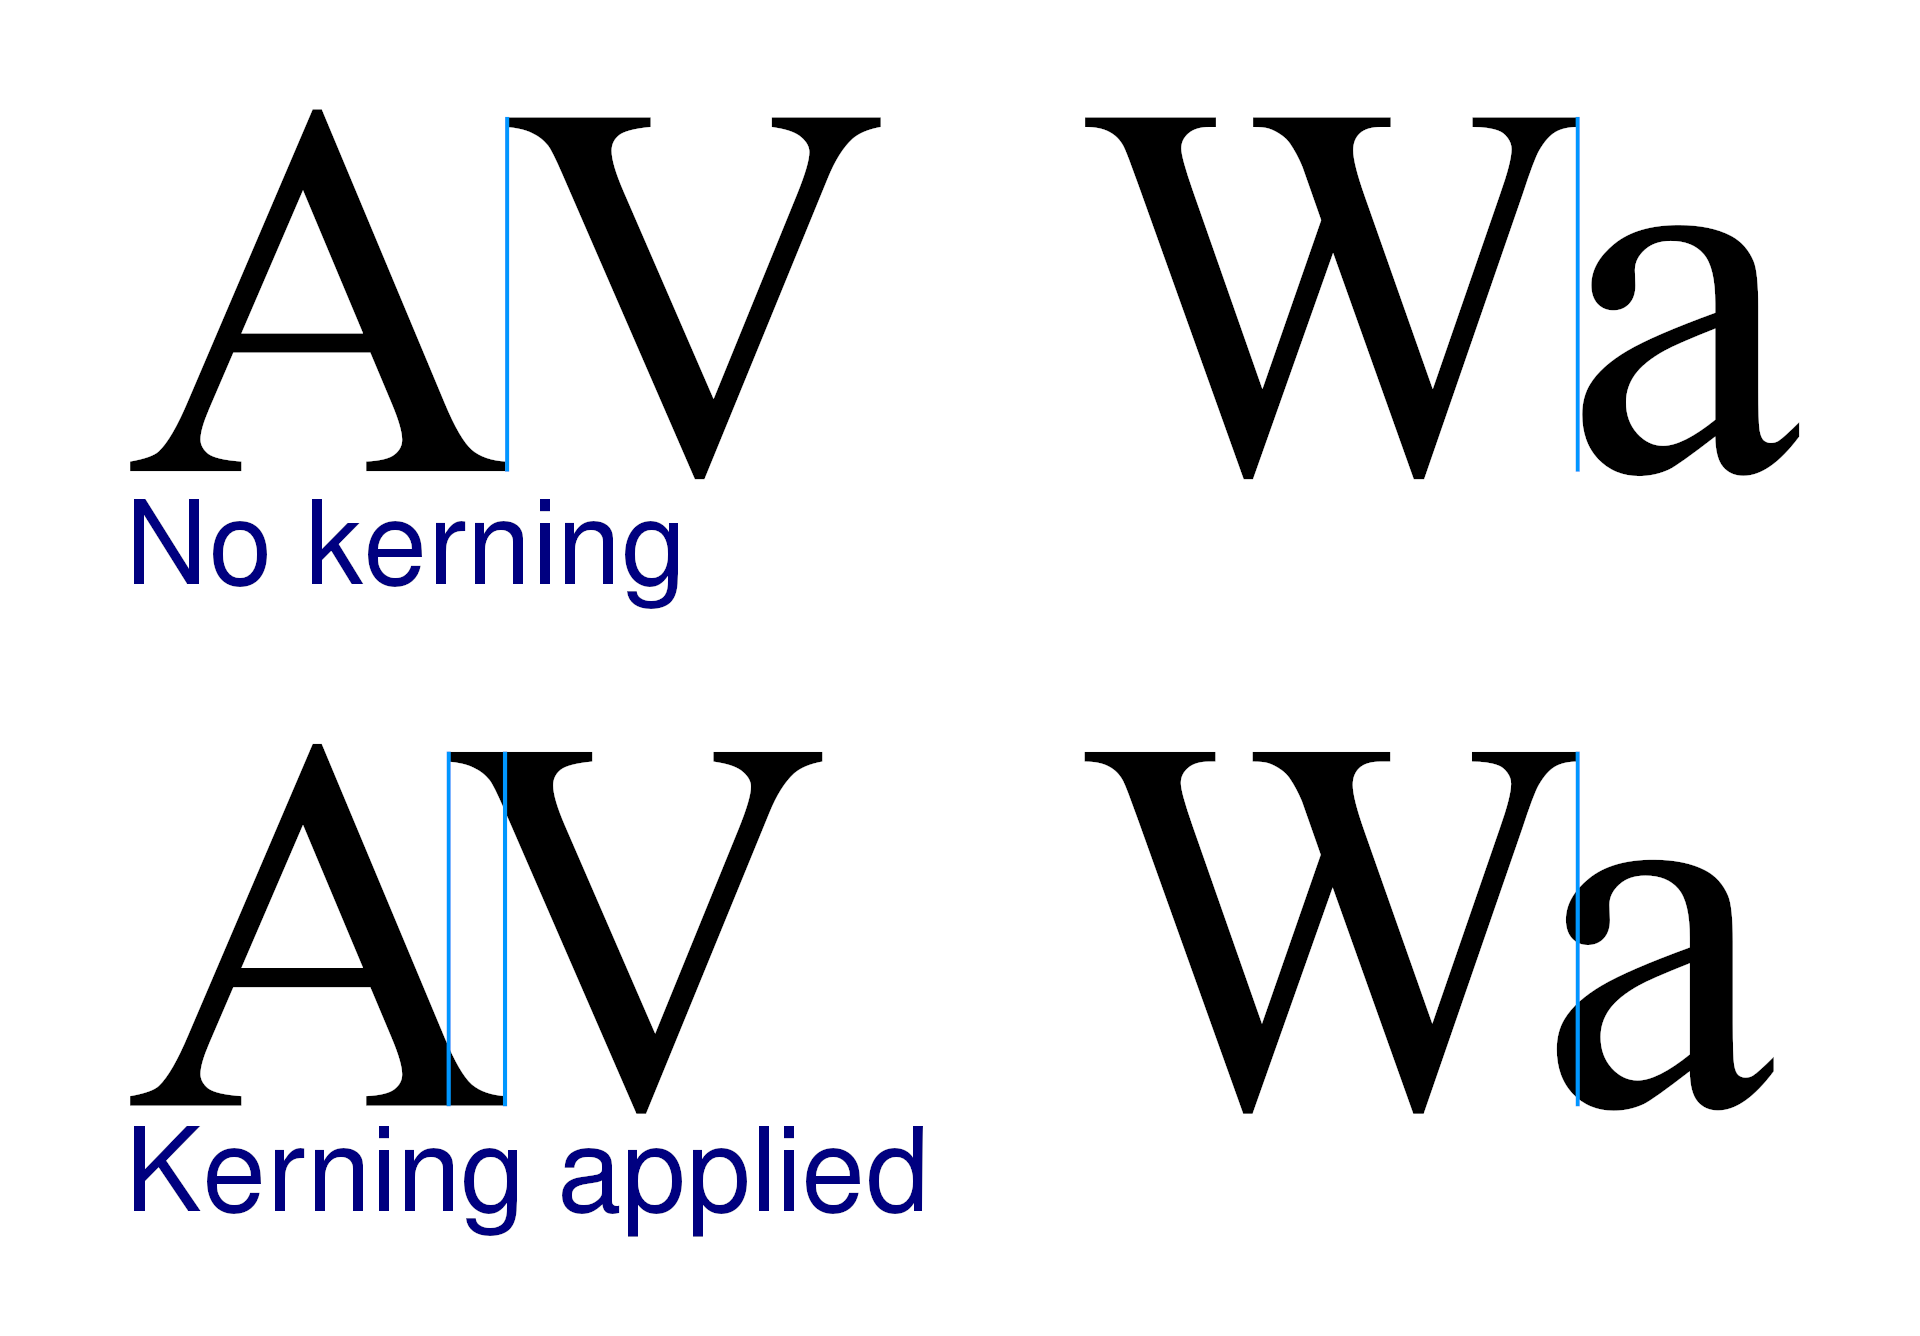
\includegraphics[width=0.25\textwidth]{images/1920px-Kerning-EN.png}
\caption{Example of kerning applied to a typeface.}
\label{kerning:fig}
\end{figure}

\begin{figure}[H]\centering
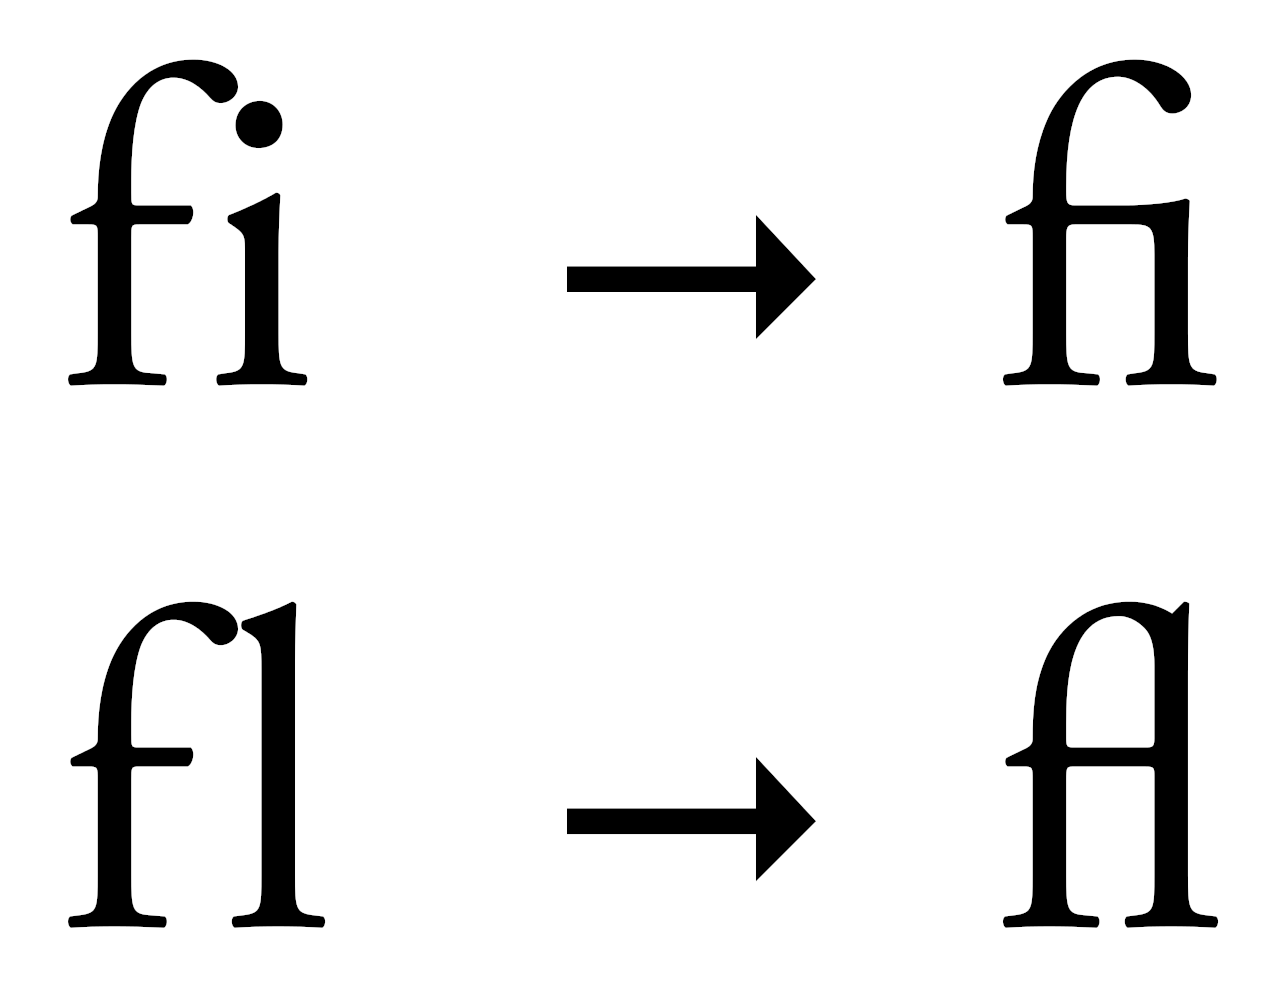
\includegraphics[width=0.25\textwidth]{images/Ligature-drawing.png}
\caption{Example of a ligature.}
\label{ligatures:fig}
\end{figure}

\textbf{While Word has several built-in tools that support multiple languages (dictionary, basic grammar check, special characters, etc.), it is not designed to handle multiple languages simultaneously.} If you want to produce, for example, a German version and an English version of your book, the best advice (using Word) would be to use two separate documents and translate and compare them paragraph by paragraph. In LaTeX, a single document can contain multiple languages.\index{multi-language project} To create a multi-language project, you can put each paragraph of the second (or third) language below the original language. This makes translation\index{translation} work more manageable and reduces work for synchronization when making revisions. This is possible by a simple switch command that uses all entries marked with either one language or with another. Check the accompanying book, (\textit{Even Better Books with LaTeX the Agile Way in 2023: Streamline Your Writing Process and Connect with Readers from Day One}, \url{https://amzn.to/3GCEGen}) for more details.

\textbf{In LaTeX, you can add functionality to switch between e-book and print output without having to manage two separate documents.} For example, my \citetitle{PFH1E} project produces four output files: the German e-book, the English e-book, the German PDF, and the English PDF. Even if your ultimate goal is to focus on the printed version of your book, merely having a more affordable e-book version will help to increase sales as it gives your readers a choice. Those who do not have a preference for reading your book in print or as an e-book might opt for the less expensive version rather than not buying your book at all.\index{price differentiation}\index{sales}

\textbf{Because LaTeX documents are compiled, you have the option to build your document not as one huge file like in Word but as a collection of many files.} As mentioned above regarding images, you can also include text files at any part of the document (as opposed to copying the whole text into one huge file). This makes it easier to divide the work and proceed section by section versus having to locate the part you are currently working on each time you open the document. It also makes rearranging sections easier: you no longer have to copy and paste pages over pages (never being sure if you have successfully copied everything and nothing was lost). Instead, you just move the \textit{reference} to a section to another place. For example, let us assume you write a book about dogs and cats and first discuss dogs, then cats. In LaTeX, you would put each discussion into a separate file and include them in your main file like this:

\begin{lstlisting}
\input{main/aboutdogs}
\input{main/aboutcats}
\end{lstlisting}

Moving your discussion about cats to the front is done by simply switching the position in the main file:

\begin{lstlisting}
\input{main/aboutcats}
\input{main/aboutdogs}
\end{lstlisting}

\textbf{If your document contains formulas, LaTeX provides an entire scientific library of functions to edit and display them directly in the document.} While you can create basic formulas in Word, you need to use a separate program to create and embed an image for any complex mathematics. Likewise, especially nonfiction books rely heavily on citations. To manage your sources in Word, you need a separate plugin or third\hyp{}party program (like \textit{Citavi}),\index{Citavi@\textit{Citavi}} while LaTeX supports the most widely used standard \textit{BibTeX}\index{BibTex@\textit{BibTex}} for free, with no plugin required.

\babelEN{\begin{definition}{Citavi} \textit{Citavi} is a plugin for Word (see \url{https://www.citavi.com}) to manage your bibliography and citations.\end{definition}}\index{Citavi@\textit{Citavi}|textbf}

\textbf{LaTeX is open source and free} (even the online editor Overleaf\index{Overleaf@\textit{Overleaf}} is free if you can do without password protection), while you have to pay license costs for Word.

\begin{figure}[H]\centering
% Diagram comparing LaTeX with Word.
\begin{tikzpicture}

% horizontal axis
\draw[->] (0,0) -- (8,0) node[anchor=north,midway] {Document complexity};
\draw[->] (0,0) -- (0,5) node[anchor=east] {Effort};

% labels
\draw	(0,-0.5) node[anchor=north] {Letters}
		(1.5,-0.5) node[anchor=north] {Articles}
		(3,-0.5) node[anchor=north] {Papers}
		(4.5,-0.5) node[anchor=north] {Theses}
		(6,-0.5) node[anchor=north] {Books}
		(7.5,-0.5) node[anchor=north] {Book series};

\draw (8,3.5) node {Word (novels)};
\draw (6,4) node {Word (social sciences)};
\draw (4,4.5) node {Word (natural sciences)};
\draw (8,2.5) node {\LaTeX{}};

% Psis
\draw[thick,dashed] (8,3.5) parabola[bend at end] (0,0.5);
\draw[thick,dashed] (6,4) parabola[bend at end] (0,0.5);
\draw[thick,dashed] (4,4.5) parabola[bend at end] (0,0.5);
\draw[thick] (0,1) parabola[bend at end] (8,3);
\useasboundingbox (-1.5,-0.2);
\end{tikzpicture}
\caption{Comparison of Word and LaTeX depending on the complexity of the task: for natural sciences, anything more complex than articles takes more effort in Word; for social sciences, anything more complex than papers takes more effort in Word; for novels, book series take more effort in Word than in LaTeX.}
\label{latex-effort-writing-complexity:fig}
\end{figure}

Ultimately, it depends on your needs. If you want to write a complex document like a book, the advantages of LaTeX outweigh those of Word. If you want to quickly write a few pages, Word is superior. For longer and more complex books, LaTeX takes less effort (see Figure~\ref{latex-effort-writing-complexity:fig}). In this book, I will help you to get your book done and published with LaTeX using the free template provided with the book.\index{LaTeX@\textit{LaTeX}!free book template}

\begin{figure}[H]\centering
\resizebox{\textwidth}{!}{\begin{tabular}{p{.2\textwidth}|p{.4\textwidth}|p{.4\textwidth}}
\hline
&\textbf{Word}&\textbf{LaTeX}\\\hline
Editor&``what you see is what you get''&source file is compiled\\\hline
Compatibility&dependent on editor&independent of editor\\\hline
Graphics&simple inbuilt editor, mouse-based&powerful but complex editor, text-based\\\hline
Typography&optimized for speed&optimized for quality\\\hline
Style&inbuilt style&separate style document\\\hline
Multi-platform&only via export&possible with scripting\\\hline
Refresh&some elements need manual refresh&everything is refreshed with each compile\\\hline
Formulas&basic support needs external tools&complete support\\\hline

\end{tabular}}
\caption{Comparison of Word and LaTeX}
\label{comparisonwordlatex:fig}
\end{figure}

\textbf{Summary:} Word is great for quickly writing a few pages, while LaTeX is better for more complex documents such as books. LaTeX provides better typography, graphics, compatibility, and multi-platform support than Word, but it requires learning the commands and therefore using LaTeX might take longer to create a document.
\newpage
% %%%%%%%%%%%%%%%%%%%%%%%%%%%%%%%%%%%%% 
% Check out the accompanying book, Even Better Books with LaTeX the Agile Way in 2023, for a discussion of the template and step-by-step instructions. https://amzn.to/3HqwgXM https://leanpub.com/eBBwLtAW/
% The template was originally created by Clemens Lode, LODE Publishing (www.lode.de), on 1/1/2023. Feel free to use this template for your book project! 
% I would be happy if you included a short mention in your book in order to help others to create their own books, too ("Book template based on \textit{Even Better Books with LaTeX the Agile Way in 2023} by Clemens Lode").
% Contact me at mail@lode.de if you need help with the template or are interested in our editing and publishing services.
% And don't forget to follow us on Instagram! https://www.instagram.com/lodepublishing/ https://www.instagram.com/betterbookswithlatex/
%%%%%%%%%%%%%%%%%%%%%%%%%%%%%%%%%%%%%

%%%%%%%%%%%%%%%%%
% This is an excerpt from the accompanying book, Even Better Books with LaTeX the Agile Way in 2023. https://www.amazon.com/Better-Books-LaTeX-Agile-Book-ebook/dp/B0BMZJ5LF7
%%%%%%%%%%%%%%%%%


\chapter{Generate Your First E-book}\label{generateyourfirstebook:cha}

\textit{So\dots{} how do we use LaTeX? What do we need to install, set up, etc.? And just how do we use LaTeX to create an e-book?} For now, we will focus on getting you started generating a PDF and e-book. Later, in Chapter~\ref{fillingthetemplate:cha}, we will go step by step through the process of copying your book from your text source (e.g., Word) to the template.

\section{LaTeX Support}\label{latexhelp:sec}

While we have tested the template that comes with this book several times, you will likely encounter an issue not discussed here. Creating a document in LaTeX \textit{is} more complex than doing so in Word, but even in Word, there are issues you might run into where the solution is not immediately apparent.\index{LaTeX@\textit{LaTeX}!support} 

If you encounter any error or have a question about LaTeX as it is used in the template, please do not hesitate to contact us. The question and the answer might be added to an FAQ for other readers. We offer free support if you provide us with a link to your Overleaf project. For major changes, one of our LaTeX developers can help you at an affordable rate. But most issues can probably be solved immediately and at no cost (``You forgot to close the parentheses,'' ``You need to load package X,'' ``Your graphics file is corrupt,'' etc.). Simply contact us at \textbf{mail@lode.de} and we will see what we can do!

For general LaTeX questions, you can also check out the community at \url{https://tex.stackexchange.com}.\index{LaTeX@\textit{LaTeX}!support!community} If you post a brief (but working) example with LaTeX code with which you are having a problem, the community can usually provide high-quality advice. If you encounter specific technical issues with the tex4ebook, you can also check whether there are open issues on the website of the tex4ebook maintainer: \url{https://github.com/michal-h21/tex4ebook}.


\section{Signing up at Overleaf}

Before we start, yes, setting up LaTeX the first time is more complicated than writing a letter in Word. But there are many solutions available that allow you to use LaTeX without much hassle. One of those solutions is Overleaf\index{Overleaf@\textit{Overleaf}}, which I am using for writing this very book (and all my other books). Overleaf is a collaborative online editor and project manager for LaTeX documents. It is available free for smaller projects that do not require password protection. If you want to keep your LaTeX code private, I recommend the Pro upgrade, which also adds full project history, access management, priority support, and support for larger projects. 

\textit{If your goal is to try things out and work on your book with a professional editor, you do not have to spend money on Overleaf for private projects or larger projects. We can host the project on our Overleaf account and manage everything for you. Drop us a message at mail@lode.de!}

\babelEN{\begin{definition}{Overleaf} \textit{Overleaf} is an online editor and project manager for LaTeX documents. It manages your project with a versioning system and automatically compiles your LaTeX code into PDF and (with some help) HTML. It is free for public projects and does not require installation or setup. You can get an account here: \url{https://www.overleaf.com}.\end{definition}}\index{Overleaf@\textit{Overleaf}|textbf}


Overleaf requires no installation.\index{Overleaf@\textit{Overleaf}!features} Just register an account, use my template, fill in your text, and you are ready to download the necessary files for creating a print book or e-book. If you are using a different LaTeX website or your own local installation, a different configuration might be required.\index{Overleaf@\textit{Overleaf}!register}\index{Overleaf@\textit{Overleaf}!sign up} To register an account on Overleaf\index{Overleaf@\textit{Overleaf}}, simply go to \url{https://www.overleaf.com}, enter your email and password, confirm the email, and log into your Overleaf account at \url{https://www.overleaf.com} clicking on \textbf{Log In}.


\section{Copy the Template}\label{copytemplate:sec}

\textit{If you do not want to use the template, check out the appendix of the accompanying book, (\textit{Even Better Books with LaTeX the Agile Way in 2023: Streamline Your Writing Process and Connect with Readers from Day One}, \url{https://amzn.to/3GCEGen}).}


Once you have your account, you have two options to get the template:

\begin{itemize}
\item go to \url{https://tinyurl.com/latextemplate2023}; or 
\item go to \url{https://www.overleaf.com/latex/templates}, searching for \textbf{Book Template for Amazon KDP, Leanpub, and Google Play (e-book and PDF) 2023}\index{template! copying}, clicking on the entry, and pressing \textbf{Open as Template}. Note that there is an earlier version available as well. Make sure you get the 2023 version!\index{template}
\end{itemize}

Once copied, you can access the template via your Overleaf project view (go to \url{https://www.overleaf.com} and click on \textbf{Projects}\index{Overleaf@\textit{Overleaf}!template} or go directly to \url{https://www.overleaf.com/project}); your new project should be listed there. 

The template itself needs to be adapted, of course\emdash{}after all, it is \textit{your} book, not mine. But for now, let us focus first on how to get from the template to a book. 

So, navigate to your project view (\url{https://www.overleaf.com}, \textbf{Projects}) and click on the new project \textbf{Book Template for Amazon KDP, Leanpub, and Google Play (e-book and PDF) 2023}. In the opened window, you should see a menu bar at the top with the \textbf{Menu} button that opens the options for the project. On the right, you will see a preview of the PDF output. Remember what I mentioned at the beginning of the book: LaTeX is not a ``what you see is what you get'' editor. Instead, whatever you write has to be compiled into a PDF. Hence, you have the actual editing window in the middle (horizontally) and the separate output window on the right side of the screen.

\begin{figure}[H]\centering
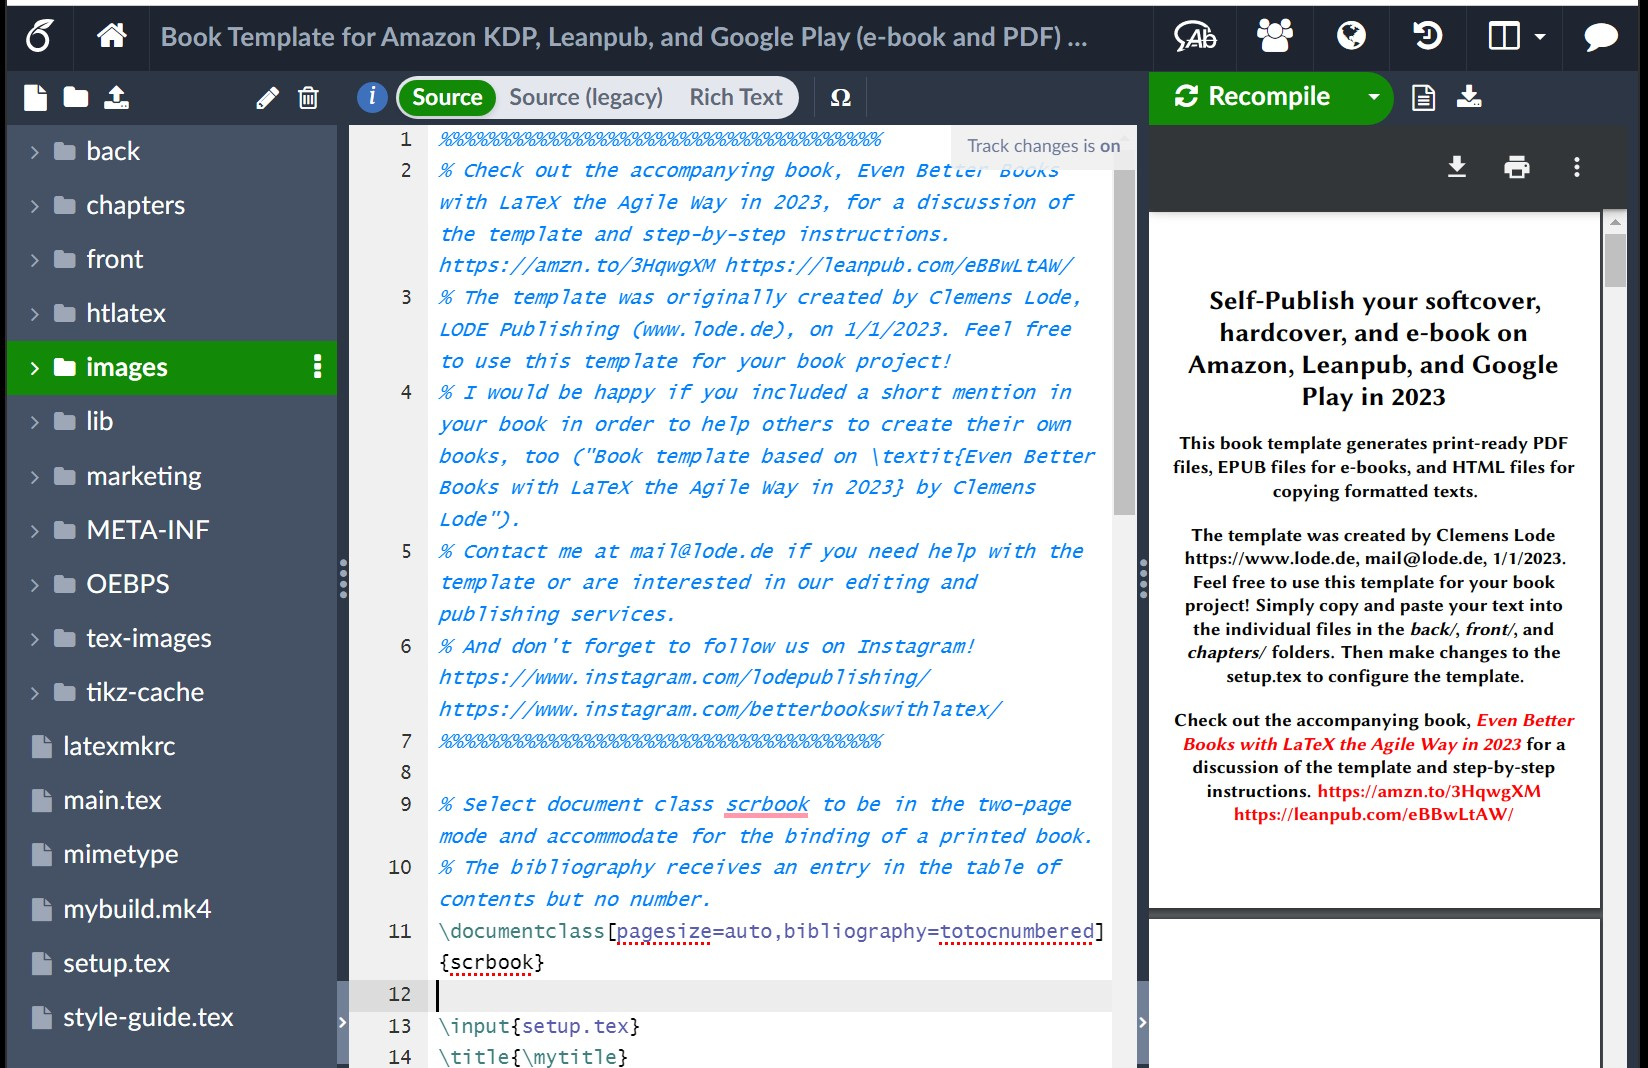
\includegraphics[width=\textwidth]{images/overleaf.jpg}
\caption{The project screen in Overleaf.}
\label{overleaf:fig}
\end{figure}



\section{Create a PDF}\label{createpdfoutput:sec}

The template is set up to produce both EPUB and PDF files.\index{template!EPUB output} The EPUB files can later be converted into formats that can be read by a Kindle e-book reader, while the PDF files can be used for printing or reading on a computer screen. In addition, there is an option to turn your LaTeX project into a HTML file to be used for easy copy and paste. For now, let us first create a PDF.\index{PDF!create}\index{create PDF}

Click on the \textbf{Menu} button at the top left. A new panel shows up (see Figure~\ref{projectsettings:fig}). In the \textbf{Settings} section, click on the drop-down menu right of \textbf{Compiler}. We want the PDF output\index{PDF!output}, so select \textbf{XeLaTeX} and select \textbf{2022} as the \textbf{TeX Live version}.

\begin{figure}[H]\centering
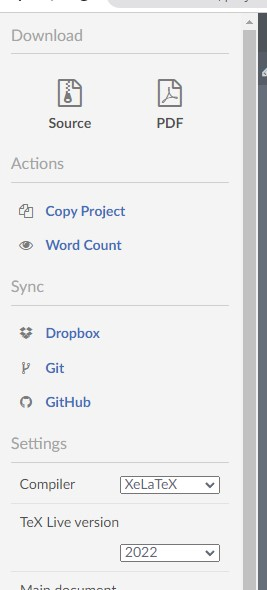
\includegraphics[width=0.4\textwidth]{images/projectsettings.jpg}
\caption{The project settings screen in Overleaf.}
\label{projectsettings:fig}
\end{figure}

\begin{definition}{XeLaTeX} \textit{XeLaTeX} is a LaTeX typesetting engine with an extended font, as well as UTF-8 encoding (for special characters) support. It takes longer to compile with \textit{XeLaTeX} than with the more basic \textit{pdfLaTeX}.\end{definition}\index{XeLaTeX@\textit{XeLaTeX}|textbf}





To download the PDF\index{PDF!download} of the \textit{XeLaTeX} output, simply click on the third symbol (\textbf{Download PDF}, the second symbol to the right of \textbf{Recompile} in the PDF view, see Figure~\ref{downloadpdf:fig}).


\begin{figure}[H]\centering

\includegraphics[width=0.4\textwidth]{images/downloadPDF.jpg}
\caption{Download the PDF via the PDF view.}
\label{downloadpdf:fig}
\end{figure}


Alternatively, you can click on \textbf{Menu} on the top left and click on \textbf{PDF} (see Figure~\ref{downloadpdfmenu:fig}).

\begin{figure}[H]\centering

\includegraphics[width=0.4\textwidth]{images/downloadPDF2.jpg}
\caption{Download the PDF via the Menu.}
\label{downloadpdfmenu:fig}
\end{figure}

Done! Your first PDF. This PDF could be used to upload to on-demand book services like Amazon's KDP.


\section{Create the EPUB Output}\label{createhtmlloutput:sec}

To create the EPUB file, we need to switch from \textit{XeLaTeX} to \textit{pdfLaTeX} output.\index{PDF!switch to EPUB output}\index{EPUB!switch to PDF output} For this, click on the \textbf{Menu} button at the top left, and this time, select \textit{pdfLaTeX} in the \textbf{Settings} section, in the drop-down menu to the right of \textbf{Compiler} (see Figure~\ref{switchpdflatex:fig}).

\begin{definition}{pdfLaTeX} \textit{pdfLaTeX} is a basic LaTeX typesetting engine that translates LaTeX documents directly into PDFs or HTML files (with the help of \textit{TeX4ht}).\end{definition}\index{pdfLaTeX@\textit{pdfLaTeX}|textbf}

\begin{figure}[H]\centering
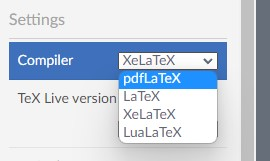
\includegraphics[width=0.4\textwidth]{images/switchpdflatex.jpg}
\caption{Switch to EPUB generation by changing the compiler in the Menu to pdfLaTeX.}
\label{switchpdflatex:fig}
\end{figure}

Next, on the left side, scroll down to \textit{latexmkrc} (see Figure~\ref{latexmkrc:fig}).

\begin{figure}[H]\centering
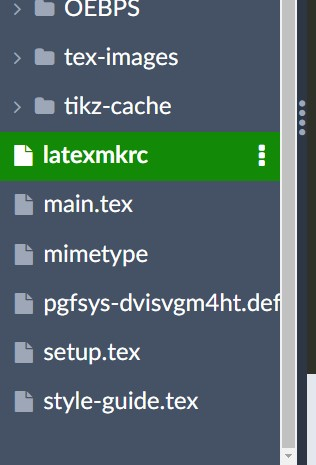
\includegraphics[width=0.4\textwidth]{images/latexmkrc.jpg}
\caption{Click here to select the \textit{latexmkrc} file.}
\label{latexmkrc:fig}
\end{figure}

There, remove the ``\#'' in front of this line (first option):

\begin{lstlisting}
# system("tex4ebook -j output -c htlatex/enumerate-fix main");
\end{lstlisting}

If you are switching back to XeLaTeX, remember to comment out this line again (add a ``\#'').

Switching the output requires you also to recompile your project. For this, click on \textbf{Recompile} in the menu above the preview window on the right (see Figure~\ref{recompile:fig}).


\begin{figure}[H]\centering

\includegraphics[width=0.4\textwidth]{images/recompile.jpg}
\caption{Click here to recompile the project.}
\label{recompile:fig}
\end{figure}

Before continuing, wait until the compilation is finished. If you encounter a problem here (and a little red box with a number appears on the document icon right beside \textbf{Recompile}, see Figure~\ref{error:fig}), please contact me at \textbf{mail@lode.de} and I will help you as soon as possible to fix the issue.\index{recompile}\index{refresh} A possible fix (especially after switching compilers) is clicking on ``Logs and output files'', then on the red \textbf{Clear cached files} button, and then again on \textbf{Recompile}.

\begin{figure}[H]\centering
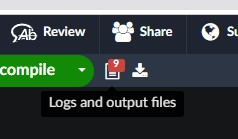
\includegraphics[width=0.4\textwidth]{images/error.jpg}
\caption{A red box with a number on the document icon indicates an error.}
\label{error:fig}
\end{figure}

If no number appears or if there are only warnings (orange box), you can proceed with the download.\index{error!compilation}\index{recompile} 

\section{Download and Convert EPUB to Kindle}\label{converthtmltokindle:sec}
\index{EPUB!convert to Kindle}

We need another tool to publish the e-book on Amazon, namely the \textit{Kindle Previewer}.\index{Kindle Previewer@\textit{Kindle Previewer}} Go to \url{https://www.amazon.com/Kindle-Previewer/b?node=21381691011} and scroll down to the download links. If the link is unavailable or broken, simply search for \textbf{Amazon Kindle Previewer} using a search engine. Once downloaded, start the installation. It will associate EPUB files with Kindle Previewer, meaning you need only to download the EPUB files to convert them.

\babelEN{\begin{definition}{Kindle Previewer} \textit{Kindle Previewer} is a Windows and MAC tool to load HTML and EPUB files and convert them into KPF and MOBI files for upload to Amazon. The tool also allows you to preview the file as a customer would see it on a Kindle eReader.\end{definition}}\index{Kindle Previewer|textbf}

For downloading the e-book,\index{template!e-book!downloading} you have to download the \textbf{EPUB} file by clicking on the \textbf{Logs and output files} icon at the top of the right window, scrolling all the way down to \textbf{Other logs \& files}, and selecting the \textbf{output.epub} entry, see Figure~\ref{downloadepub:fig}).\index{EPUB!download} 

\begin{figure}[H]\centering
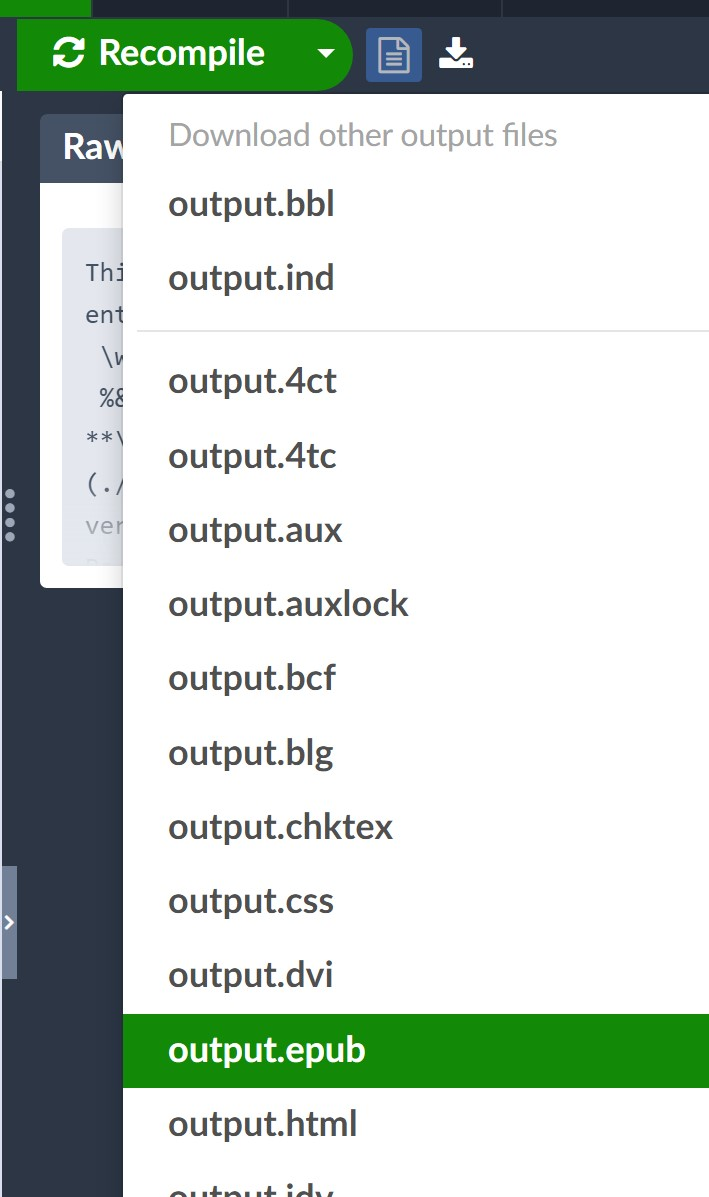
\includegraphics[width=0.65\textwidth]{images/downloadEPUB.jpg}
\caption{The EPUB file with the HTML output, style information, and images can be downloaded in the ``Logs and output files'' screen at the very bottom.}
\label{downloadepub:fig}
\end{figure}

A download with the EPUB file should start now, and, once completed, Kindle Previewer should start automatically (or you first need to click on the file, depending on your browser's configuration). If you want to convert an EPUB file already downloaded on your computer, start the Kindle Previewer manually, select \textbf{File / Open Book} (see Figure~\ref{kindlepreviewer:fig}), browse to the directory where you have the EPUB file, and press \textbf{Open}. This starts the conversion process.

\begin{figure}[H]\centering
\adjustbox{max height=.35\textheight}{
    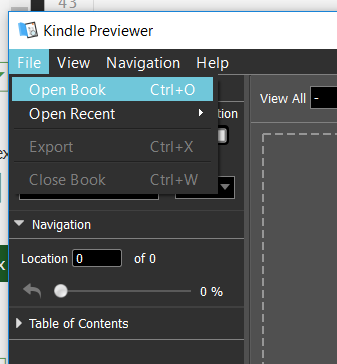
\includegraphics{images/kindlepreviewer.png}
}
\caption{Importing the EPUB file in Kindle Previewer to convert it into a KPF or MOBI format.}
\label{kindlepreviewer:fig}
\end{figure}

Note that if you also want the HTML output (for example, to copy contents), check out the appendix of the accompanying book, (\textit{Even Better Books with LaTeX the Agile Way in 2023: Streamline Your Writing Process and Connect with Readers from Day One}, \url{https://amzn.to/3GCEGen}).


\section{Converting EPUB to KPF with the Kindle Previewer}

\textit{For general information about the Kindle Previewer, check out its homepage at \url{https://kdp.amazon.com/en_US/help/topic/G202131170}}

Depending on the book size, converting an EPUB file to a KPF file might take a moment. During conversion, you will see the ``Converting your book to Kindle format'' message on the screen. Once finished, a virtual Kindle reader\index{Kindle!preview} should show up where you can browse through your book. If you are happy with how the contents look, press \textbf{File / Export} in the menu, and press \textbf{Export}. For the name of the exported file, I recommend including the current date to prevent confusion when uploading (for example, \textit{ebbwltaw-01012023.kpf}). You can select different output formats. Choose the (pre-selected) format \textbf{Books(.kpf)}, which is the newest and most compatible format.

A message box should appear that reads ``Book is successfully exported here.'' You can safely ignore the warning message ``Enhanced typesetting is enabled for the book being previewed, but it is not supported in the exported file.'' This refers only to the fact that any fonts you are using in your LaTeX project are ignored and replaced by the respective fonts of the e-book reading device. Now you have a KPF file\index{KPF!convert from EPUB} that you can use later to upload to Amazon's KDP platform and release it directly as an e-book on Amazon. I discuss the details in the accompanying book, (\textit{Even Better Books with LaTeX the Agile Way in 2023: Streamline Your Writing Process and Connect with Readers from Day One}, \url{https://amzn.to/3GCEGen}), but in essence, that is the entire publishing process, at least from the technical side.



\section{Versioning}\label{versioning:sec} \index{versioning}

\textbf{Before you continue:} while you are learning LaTeX, you should create a backup\index{backup!create}\index{Overleaf@\textit{Overleaf}!backup} whenever your project compiles successfully. You can click on \textbf{History} (top menu, see Figure~\ref{versions:fig}), then on \textbf{All history}, then on \textbf{View single version}, then on \textbf{Label this version}, then enter a name for the backup.

\begin{figure}[H]\centering
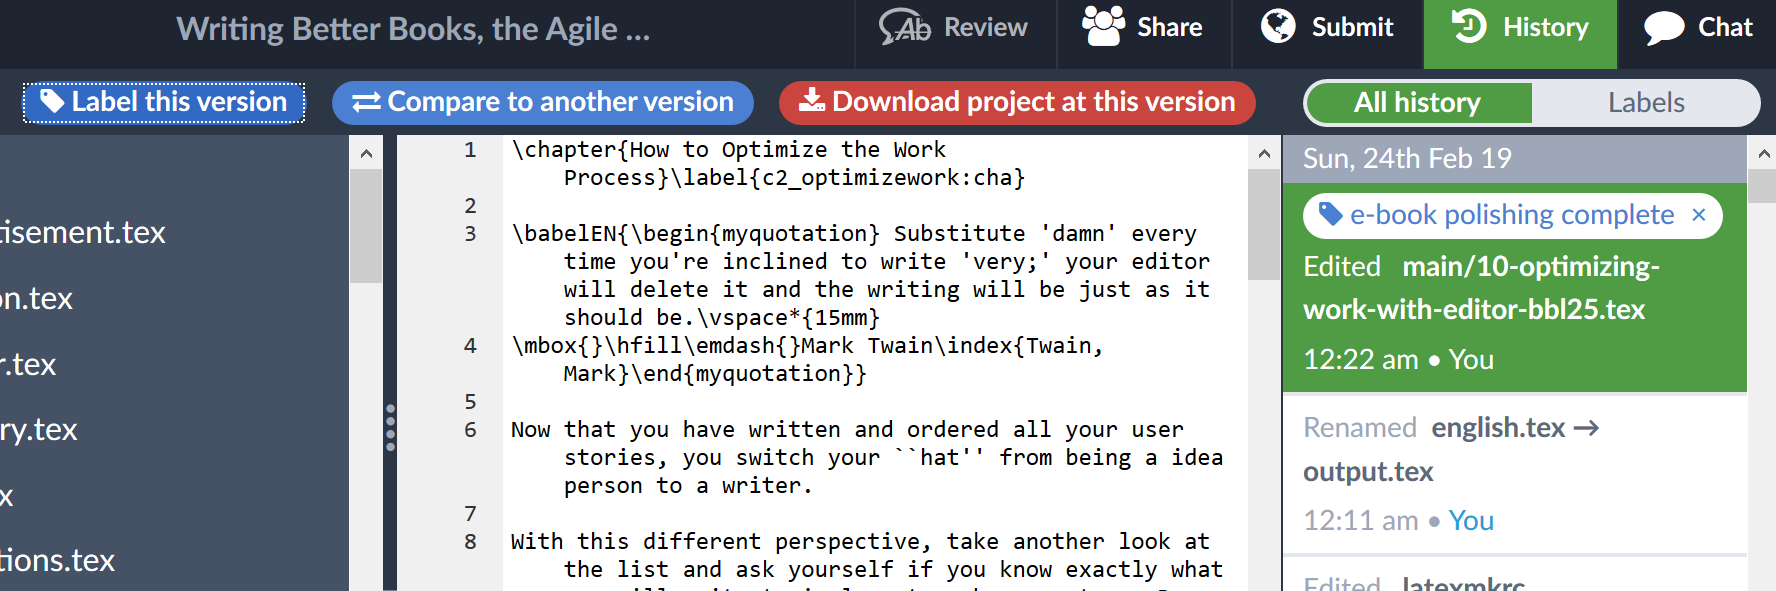
\includegraphics[width=0.95\textwidth]{images/versions.png}
\caption{Setting the name of the current version of the book for later reference.}
\label{versions:fig}
\end{figure}

It is best to name each backup\index{backup!naming} by the milestone you have reached so that you later know at what point you have made the backup. For example, after polishing the files for an e-book release (but before polishing it for print), you could name it ``e-book polishing complete.''

You can always go back to a previous version and compare your changes. Click on \textbf{History}, then on \textbf{Compare to another version}, then on \textbf{Labels}, and then on a file in the list on the left side with a note ``edited'' right beside it. That being said, you do not have to save as you write. Your latest changes are always saved automatically. 

\textbf{Summary:} This chapter showed you how to generate a PDF file and an EPUB file from the LaTeX template. You signed up at Overleaf, copied the template, switched the output from XeLaTeX to pdfLaTeX, downloaded the PDF and EPUB files, converted the EPUB to KPF with the Kindle Previewer, and created backups of your project.\newpage
% %%%%%%%%%%%%%%%%%%%%%%%%%%%%%%%%%%%%% 
% Check out the accompanying book, Even Better Books with LaTeX the Agile Way in 2023, for a discussion of the template and step-by-step instructions. https://amzn.to/3HqwgXM https://leanpub.com/eBBwLtAW/
% The template was originally created by Clemens Lode, LODE Publishing (www.lode.de), on 1/1/2023. Feel free to use this template for your book project! 
% I would be happy if you included a short mention in your book in order to help others to create their own books, too ("Book template based on \textit{Even Better Books with LaTeX the Agile Way in 2023} by Clemens Lode").
% Contact me at mail@lode.de if you need help with the template or are interested in our editing and publishing services.
% And don't forget to follow us on Instagram! https://www.instagram.com/lodepublishing/ https://www.instagram.com/betterbookswithlatex/
%%%%%%%%%%%%%%%%%%%%%%%%%%%%%%%%%%%%%

%%%%%%%%%%%%%%%%%
% This is an excerpt from the accompanying book, Even Better Books with LaTeX the Agile Way in 2023. https://www.amazon.com/Better-Books-LaTeX-Agile-Book-ebook/dp/B0BMZJ5LF7
%%%%%%%%%%%%%%%%%

\chapter{Filling the Template}\label{fillingthetemplate:cha}

Now that you have experienced the steps of creating documents with the template, you can start to add content to them. In this section, we will go through each file of the template (\url{https://tinyurl.com/latextemplate2023}) and give you a ``to do'' list of items you can work on one by one\emdash{}from the title to the appendix.

One way to understand the structure of a book is to imagine how books were created before the digital age.\index{book!structure} Imagine various groups of people working on the book and handing over the results to the next group. At the beginning of this process, there is the core material that makes up most of the book: the individual chapters and sections. Those are surrounded by the front and back matter, which consist of several layers. The author hands the text of the \textit{chapters} over to the editor\index{editor}, together with a note introducing the author's work (the \textit{preface})\index{preface}. The editor adds the \textit{table of contents}\index{table of contents}, the \textit{index}\index{index}, \textit{bibliography}\index{bibliography}, \textit{quotation sources}\index{quotation!sources}, and maybe an \textit{appendix}\index{appendix} (containing summaries from throughout the book), and hands the book over to the \textit{publisher}. 

The publisher\index{publisher} adds information to the book, too. That is, first the \textit{publisher} page itself with the year of publication, ISBN number, copyright note, and publisher name, and then a description of how the book was created and, for example, how the reader can contact the publisher with any questions (the \textit{foreword})\index{foreword}. All the parts are then put into an envelope (consisting of the \textit{series title}\index{series title} and \textit{half title}\index{half title}) and handed over to the cover designer. The cover designer\index{cover designer} creates the cover\index{cover} (front, back, and spine), packages it together with the book into another envelope (consisting of the \textit{title page}\index{title} including the cover picture), and hands it to the printer. 

\section{Main Document /main.tex}\label{entrypoint:sec}

The main document of an Overleaf project is the file in which Overleaf starts processing your project. When looking to make major changes like adding, rearranging, or removing sections and chapters, this is also the place for you to look first. 

By default, the main document of an Overleaf project is \textit{main.tex}. You can find this file on the left side in the project file overview.\index{/main.tex}. You can change the project's main document in Overleaf by clicking on ``Menu'' under ``Settings / Main document.''


\section{Global Setup}\label{globalsetup:sec}

The first file included in \textit{main.tex} is \textit{setup.tex}. This file defines all the global parameters of your book\emdash{}for example, the book's dimensions, the book's author, and the book's title. In the left project window, scroll down until you see \textit{setup.tex}.\index{/setup.tex} Click on it and start editing the file:


\subsection{Title Information}

\begin{itemize}
\item Replace ``The Title'' with your book title;
\item Replace ``The Subtitle'' with your book subtitle;
\item Replace ``Publishing Company'' with your publishing company's name; and
\item Replace ``Location of the Publishing Company (city)'' with your publishing company's location (the city), and ``\url{https://www.lode.de}'' with the URL (using https://) of your publishing company's website.
\end{itemize}

About the last two points, if you do not own a company, put in your own name and address and leave the URL empty. Note that from a legal standpoint, the exact requirements for providing the address depend on the country where you are publishing the book. Writing down all the information puts you on the safe side; if you want privacy, you must check what is required by law (and perhaps consider a P.O.~box). Alternatively, just contact us (mail@lode.de), and maybe we can publish your book, and you will not have to worry about any paperwork.

We also need two cover versions,\index{cover!requirements} one for the e-book (JPG: low resolution, lossy compression) and one for print (PNG: high resolution, lossless compression). The reason is that (at least on platforms like Amazon) your profits for each e-book shrink depending on the file size. In 2023, this download charge for Amazon.com was around \${}.15 per MB, so a 10 MB e-book would reduce your profit per book by nearly \${}1.50 (check \url{https://kdp.amazon.com/en_US/help/topic/G200634500} for current prices depending on the country of publication). For print, the file size can be ignored, and thus, the image quality can and should be as high as possible.\index{cover!resolution}\index{e-book!resolution}\index{resolution} 

Rename both versions of your cover (PNG and JPG) \textit{cover.png} and \textit{cover.jpg} and upload them into the \textit{images} folder. If you want to use different filenames, simply upload your cover files and replace the file name entries in the \textit{setup.tex}\index{/setup.tex} and \textit{output.opf} file.

For the latter, see the accompanying book, (\textit{Even Better Books with LaTeX the Agile Way in 2023: Streamline Your Writing Process and Connect with Readers from Day One}, \url{https://amzn.to/3GCEGen}).

\textit{If you do not have a cover file, skip this step. I discuss cover creation in the accompanying book, (\textit{Even Better Books with LaTeX the Agile Way in 2023: Streamline Your Writing Process and Connect with Readers from Day One}, \url{https://amzn.to/3GCEGen}).}

To upload the cover files, click on the \textit{images} directory in the left project window, click on the arrow, select \textbf{Upload}, and then ``select from your computer.'' If the files already exist, they will be overwritten. The most straightforward approach is to rename your cover file to fit the existing template; otherwise, you have to change the corresponding entry in the \textit{setup.tex} file:

\begin{lstlisting}
    \newcommand{\coverImage}{images/cover.jpg}
    \newcommand{\hiresCoverImage}{images/cover.png}
\end{lstlisting}



\subsection{Publisher Information}

To set up the publisher information page:

\begin{itemize}
\item Replace ``Your email address'' with your email address;
\item Replace ``First'' with the edition number;
\item Replace the three ISBN numbers with your e-book's, softcover's, and hardcover's ISBN numbers; 
\item Replace ``Your editor's name'' with your editor's name;
\item Replace ``Your designer's name'' with your book cover designer's name;
\item Replace ``Your image sources'' with your image and icon source (e.g., ``Shutterstock''), including its license type; and
\item Replace ``Your newsletter email'' and ``Your newsletter URL'' with the email and URL (using https://) where people can subscribe to your newsletter.
\end{itemize}

You can skip replacing the ISBN numbers for now. What numbers to enter here depends on what publishing service you use. For example, for Amazon, see the accompanying book, (\textit{Even Better Books with LaTeX the Agile Way in 2023: Streamline Your Writing Process and Connect with Readers from Day One}, \url{https://amzn.to/3GCEGen}) for more details.


\subsection{About the Author}

Next, fill in information about you (the author):

\begin{itemize}
    \item Replace ``Your name'' with your name;
    \item Replace ``Your city'' with your location;
    \item Replace ``Your country'' with the country where you live;
    \item Replace ``Preface date'' with the date when you have written the preface (and finalized the book); and
    \item If you want, upload a high-resolution (\textit{author.png}) and a low-resolution picture (\textit{author.jpg}) of the author into the \textit{images} folder. Also, uncomment the ``\%\\useAuthorImagetrue'' line.
\end{itemize}




\subsection{Series Title}

If your book is part of a series, uncomment the ``\%\\seriestrue'' line by removing the ``\%'' and filling out the titles of the parts and the name of the book series. If it is not the first book of the series, comment out the ``\\firstBookOfSeries'' line by adding a ``\%'' and filling out the number and title of the previous part of the series, and uploading the images of the previous part. In the accompanying book, (\textit{Even Better Books with LaTeX the Agile Way in 2023: Streamline Your Writing Process and Connect with Readers from Day One}, \url{https://amzn.to/3GCEGen}), I discuss how to write a series. In the following paragraphs, we will assume that it is a standalone book.



\section{File Structure}\label{filestructure:sec}

Now that we have filled in the global information, we can go file by file to replace the actual text blocks. In the accompanying book, (\textit{Even Better Books with LaTeX the Agile Way in 2023: Streamline Your Writing Process and Connect with Readers from Day One}, \url{https://amzn.to/3GCEGen}), I discuss adapting the \textit{structure} of the book, meaning in which sequence the chapters are placed in the book.

\subsection{Front Matter}\label{frontmatter:sec}

In the left project window, click on the \textit{front} folder. You will see a list of several files open.

\begin{itemize}
    \item Select \textit{front/title.tex}.\index{/front/title.tex} This will be the first page of the document. Nothing needs to be done here, we filled all variable elements automatically using the \textit{setup.tex}.

    \item Next, open \textit{front/half-title.tex}\index{/front/half-title.tex}. In the print edition, this comes after the title on page 3 of the book. Here, too, nothing further needs to be edited.

    \item Next, open \textit{front/publisher.tex}\index{/front/publisher.tex}. This page is usually reserved for information about the book as a product. It lists information about when the book was produced, by whom, and how someone can reach you. If you have filled out the \textit{setup.tex} correctly, your work in this file is done.

    \item Next is the \textbf{dedication}\index{dedication} page (see \textit{front/dedication.tex}\index{/front/dedication.tex}). Here, you can thank the people who helped you create the book. This page stresses that books build on other people's work. When writing it, think of it as a letter you would send to those people. Some people just write, ``To my husband/wife/parents.'' If you see it as but a chore and want to express your gratitude to those people in person rather than in writing, you can safely leave out the dedication page. In the accompanying book, (\textit{Even Better Books with LaTeX the Agile Way in 2023: Streamline Your Writing Process and Connect with Readers from Day One}, \url{https://amzn.to/3GCEGen}), I discuss how to rearrange, add, or remove entire pages or sections.


    
    \item Another optional page is the \textbf{epigraph}\index{epigraph} page (see \textit{front/epigraph.tex}\index{/front/epigraph.tex}). This page sets the theme for the book. This can be a quote, a picture, or anything you think could fit here. Here you can be creative and put some emotion into your book, even if it might be a dry book about LaTeX and project management. In my book \citetitle{PFH1E}, I have used the epigraph to introduce the reader to the summary boxes\emdash{}insights into philosophy and linguistics\emdash{}that I have put at the end of every section. They tell a meta-story. They are the icing on the cake. For your epigraph, consider whether you want to add a particular plot or theme to your nonfiction book. The epigraph page is the perfect place to introduce this concept.

    \item Next comes the \textbf{foreword} (see \textit{front/foreword.tex}\index{/front/foreword.tex}). This is written by the publisher or you, with your self-publisher hat on. It should focus less on the book's content and instead focus on the book's production process. Encourage the reader to give you feedback and advise how he or she can contact you with an issue with the book, such as an error. Alternatively, the foreword can be written by an expert in the field as a type of endorsement. 

    \item After the foreword, it is now up to you, the author, to introduce the book in the \textbf{preface} (see \textit{front/preface.tex}\index{/front/preface.tex}). This can include how you arrived at the decision to write it, a personal note to the readers, and an ``elevator pitch,''\index{elevator pitch} a short introduction telling the reader why this book is an essential read. Try to be personal and try to stay away from sales talk or corporate speech. Add a quote by your favorite author as a finishing touch. You have already entered the information about you, the author, and the book series (if applicable) in the \textit{setup.tex}, so you are done with this file, too.

\end{itemize}

This concludes the front matter of the book. The remaining file, \textit{series-title.tex}, is discussed in the accompanying book, (\textit{Even Better Books with LaTeX the Agile Way in 2023: Streamline Your Writing Process and Connect with Readers from Day One}, \url{https://amzn.to/3GCEGen}).


\newpage\section{Main Matter}\label{mainmatter:sec}

In the folder list in the project view on the left, you will see a folder named \textit{chapters}. This is the place for the main content, with a separate file for each chapter. Inside the \textit{chapters}\index{/chapters} folder, you will find \textit{0-latex.tex}\textit{0-latex.tex}, \textit{01-advantages-latex.tex}, \textit{02-generate-first-ebook.tex}, and \textit{03-filling-template.tex}. Those are just sample files showing excerpts of this book (the first three chapters of Part 2, including this chapter). You can delete the files after adding your own material.

\begin{itemize}

\item If you already have your whole book (or portions of it) ready in one big Word (or text) file, you first need to separate the text by chapter.

\item If you have already separated your book into individual chapters, each in its own file, proceed as outlined below.

\end{itemize}

For each chapter\index{chapter}, create a new file in the \textit{chapters} directory in Overleaf. Instead of calling them \textit{first-chapter.tex}, \textit{second-chapter.tex}, etc., name them according to their actual chapter titles, preceded by the chapter number (for example, in this book project, I have named the file of this chapter \textit{03-filling-template.tex}). This way, you can more easily refer to them later. Naming the first part of a chapter file according to its chapter number (01, 02, etc.) helps with navigation, but you can use any naming convention you like (just make sure you are consistent).

Once you have identified all chapters and created the files, you need to copy the text into each chapter file. For this, simply select the text of your chapter (including the title), and copy and paste it into the corresponding \textit{.tex} file. There is a chance that the project will no longer (or only partially) compile after inserting your text. This can happen if your text already contains what Overleaf interprets as LaTeX commands. The most frequent issues are:

\begin{itemize}
\item \textbf{Percentage signs \%}\index{percentage sign}\index{\%}  \textit{They are interpreted as comments by LaTeX and are thus ignored.} Replace them with ``\textbackslash\%''
\item \textbf{Curly braces \{ \}}\index{curly braces}\index{\{\}}  \textit{They are interpreted as special commands by LaTeX.} Replace them with ``\textbackslash\{'' or ``\textbackslash\}''
\item \textbf{Dollar signs \$}\index{\$}\index{dollar sign}  \textit{They are interpreted as starting or ending a mathematical formula.} Replace them with ``\textbackslash\$\{\}''
\item \textbf{Underscores \_}\index{underscore}\index{\_}  \textit{They are used in mathematical formulas.} Replace them with ``\textbackslash\_'' or remove them altogether, especially in file, chapter, section, and figure names. It is fine to keep them as part of URLs (inside a \textbackslash url command) or code (inside a \textbackslash lstlisting environment).
\end{itemize}

\textit{Please note that there is no simple way of copying the formatting (bold, italic, font size, lists, indentation, etc.) from Word to LaTeX. In the accompanying book, (\textit{Even Better Books with LaTeX the Agile Way in 2023: Streamline Your Writing Process and Connect with Readers from Day One}, \url{https://amzn.to/3GCEGen}), I discuss how to format the text manually, especially if you already have your text formatted in Word. For any future books, I recommend that you write them in Overleaf from scratch and use the LaTeX formatting as you write.\index{chapter!organization}\index{organization}}


\section{Chapter Header}

One way of starting each chapter file is by defining the chapter title and label, and adding a quotation to set the tone of the chapter. You can reuse the code for each new chapter file by copying and pasting the following code to the top of your files:

\begin{lstlisting}
\chapter{Replace with the Chapter Name}\label{chaptername:cha}

\begin{myquotation} The perfect place for an introducing quotation.
\mbox{}\hfill \emdash{}Famous Person\index{Person, Famous}
, \citetitle{bibitem}\index{@\citetitle{bibitem}} \ifxetex\label{famousperson-bibitem-quote}\else\citep[p.~123]{bibitem}\fi
\par\end{myquotation}


\end{lstlisting}


\begin{itemize}
\item Replace ``Replace with the Chapter Name'' with your chapter title.
\item Replace ``chaptername'' with your chapter title label (no spaces, only lowercase letters).
\item Replace the quotation text, add the person's name, and (if you have it) the bibliography item. If you do not have the source, remove the following line:

\begin{lstlisting}
, \citetitle{bibitem}\index{@\citetitle{bibitem}} \ifxetex\label{famousperson-bibitem-quote}\else\citep[p.~123]{bibitem}\fi
\end{lstlisting}
\end{itemize}

There are several approaches to organizing your book's individual chapters and sections. Personally, I prefer to divide my content into small (ideally independent) slices, with each slice providing the reader with some benefit. The accompanying book, (\textit{Even Better Books with LaTeX the Agile Way in 2023: Streamline Your Writing Process and Connect with Readers from Day One}, \url{https://amzn.to/3GCEGen}) discusses the entire process from idea to publishing.


\section{Back Matter}\label{backmatter:sec}

The back matter\index{back matter} of a book typically consists of two elements: references and connecting with the author.

\begin{itemize}
    \item  By ``references''\index{references} I mean the glossary\index{glossary}, questions to reflect on about the book's contents, a summary of the main points of the book, the index, a list of image and quotation sources, and the bibliography. Whether or not you want to include the glossary, the questions, and the summary of ideas depends on the book you are writing. The index is created automatically, but it will need some work within the text of the main matter of the book, which I discuss in the accompanying book, (\textit{Even Better Books with LaTeX the Agile Way in 2023: Streamline Your Writing Process and Connect with Readers from Day One}, \url{https://amzn.to/3GCEGen}). The same applies to the bibliography.
    
    \item By ``connecting with the author'' I mean the ``About the Author''\index{/back/author.tex} section, information about your (or your publisher's) other books, an optional section about how the book was created, and a polite reminder to your readers to leave a written review online. If you want to give the book a finishing touch, end with a short quote on the last page.\index{author page} 
\end{itemize}

For the second part, let us go through the files of the template one by one.

\begin{itemize}

\item If you have other books published, the \textit{back/advertisement.tex}\index{/back/advertisement.tex} is the place you can list them. In the template, replace or remove the pictures of the book covers, and replace or remove the descriptions of the individual book entries.

\item Next, you are free to use the text in \textit{back/amazon.tex}\index{/back/amazon.tex} if you like or adapt it to your own needs, depending on where you publish the book. This is a reminder for the reader to provide you (and potential future readers) feedback.

\item For information about you, the author, open the \textit{back/author.tex}\index{/back/author.tex} file and replace the quotation text and add a short text describing your motivation, your professional background, what you are currently doing, and how to contact you.

\item Beyond the cited works and your other books, you can also direct the reader to additional book recommendations to delve deeper into the subject. For this, use the command \textbf{\textbackslash nocite}\index{\textbackslash nocite} in the \textit{back/recommended.tex}\index{/back/recommended.tex} file and list the recommended books by their book id from your bibliography file.

\item If you want to tell a story about how you created your book (if you have not already done so in the preface), you can do so in the \textit{back/thebooksstory.tex}.\index{/back/thebooksstory.tex} Use this chapter to summarize what you have learned while writing the book. This can help you to write better books in the future and might be interesting for the reader as well. Myself, I like to talk about what is going on in the background of what I do. It is up to you. The existing default text in the template describes to a reader how the book was created using the template and this book as a guide. Feel free to skip this one. In the accompanying book, (\textit{Even Better Books with LaTeX the Agile Way in 2023: Streamline Your Writing Process and Connect with Readers from Day One}, \url{https://amzn.to/3GCEGen}) I cover how to reorganize or remove individual sections.

\item Finally, replace the quote in \textit{back/last.tex}\index{/back/last.tex} with a quote of your choice in order to leave the reader with something to think about.

\end{itemize}

The remaining files in the back matter are as follows (see the accompanying book, \textit{Even Better Books with LaTeX the Agile Way in 2023: Streamline Your Writing Process and Connect with Readers from Day One}, \url{https://amzn.to/3GCEGen} for more details):

\begin{itemize}
    \item \textit{bibliography.tex}\index{/back/bibliography.tex}: The bibliography.
    \item \textit{index.tex}\index{/back/index.tex}: The index.
    \item \textit{glossary.tex}\index{/back/glossary.tex}: The glossary is added at the end of your book as a reference. You can add glossary boxes throughout your book to explain concepts. Create a separate glossary file in the \textit{chapters/glossary} directory and use \textit{input} to include them in your chapters and the glossary. Ideally, sort your glossary items in the \textit{glossary.tex} file by their name.
    \item \textit{questions.tex} and \textit{ideas.tex}\index{/back/questions.tex}\index{/back/ideas.tex}: Similar to the glossary entries, you can add questions and answers throughout your chapters and include them in the back matter as a reference. For better navigation, sort them by chapter.
    \item \textit{quotations.tex}\index{/back/quotations.tex}: If you are citing from other sources, list them in this file. This is especially helpful for e-book readers who might not have access to footnotes.
\end{itemize}


\textit{What about the table of contents?}\index{table of contents} While it is generated automatically in both LaTeX and Word, updating it in LaTeX requires no additional work. As the project files are fully compiled after each change, you do not even need to manually refresh the table of contents. We still have to organize and format the text you have pasted into the book's main matter. Once that is done, your entire table of contents will show up in the output.

That is it! Your book is finished and we can now move on to polishing. 

Chances are that a few issues have come up through the copying and writing process. \textit{That is normal!} Remember, LaTeX takes a little bit of time to learn. But once you know it, it flows like a natural language. All it takes is patience. If you hit a wall, you can create a new copy of the template and progress in smaller steps. Even better, use the backup and restore feature (see the accompanying book, \textit{Even Better Books with LaTeX the Agile Way in 2023: Streamline Your Writing Process and Connect with Readers from Day One}, \url{https://amzn.to/3GCEGen} for more details) using the top menu entry (\textbf{History}). Also, you can always contact us (mail@lode.de); we may have a quick fix for your problem. Alternatively, we could bring your book to the market together.

\textbf{Summary:} In this chapter, we went through each of the files in the template. First, we covered how to fill them. We started with the main document, \textit{main.tex}, and created a global setup using the \textit{setup.tex} file. We then filled in the front matter, main matter, and back matter. We learned how to organize chapters, create a book series, insert quotations, introduce the author, and leave the reader with something to think about. Finally, we discovered how to rearrange, add, or remove individual sections.\newpage

%%%%%%%%%%%%%%%%%
% Back matter
%%%%%%%%%%%%%%%%%
\backmatter

% %%%%%%%%%%%%%%%%%%%%%%%%%%%%%%%%%%%%% 
% Check out the accompanying book, Even Better Books with LaTeX the Agile Way in 2023, for a discussion of the template and step-by-step instructions. https://amzn.to/3HqwgXM https://leanpub.com/eBBwLtAW/
% The template was originally created by Clemens Lode, LODE Publishing (www.lode.de), on 1/1/2023. Feel free to use this template for your book project! 
% I would be happy if you included a short mention in your book in order to help others to create their own books, too ("Book template based on \textit{Even Better Books with LaTeX the Agile Way in 2023} by Clemens Lode").
% Contact me at mail@lode.de if you need help with the template or are interested in our editing and publishing services.
% And don't forget to follow us on Instagram! https://www.instagram.com/lodepublishing/ https://www.instagram.com/betterbookswithlatex/
%%%%%%%%%%%%%%%%%%%%%%%%%%%%%%%%%%%%%


\chapter{TikZ Examples}\label{tikz-examples:cha}

\begin{figure}
\centering
% Diagram comparing LaTeX with Word.
\begin{tikzpicture}

% horizontal axis
\draw[->] (0,0) -- (8,0) node[anchor=north,midway] {Document complexity};
\draw[->] (0,0) -- (0,5) node[anchor=east] {Effort};

% labels
\draw	(0,-0.5) node[anchor=north] {Letters}
		(1.5,-0.5) node[anchor=north] {Articles}
		(3,-0.5) node[anchor=north] {Papers}
		(4.5,-0.5) node[anchor=north] {Theses}
		(6,-0.5) node[anchor=north] {Books}
		(7.5,-0.5) node[anchor=north] {Book series};

\draw (8,3.5) node {Word (novels)};
\draw (6,4) node {Word (social sciences)};
\draw (4,4.5) node {Word (natural sciences)};
\draw (8,2.5) node {\LaTeX{}};

% Psis
\draw[thick,dashed] (8,3.5) parabola[bend at end] (0,0.5);
\draw[thick,dashed] (6,4) parabola[bend at end] (0,0.5);
\draw[thick,dashed] (4,4.5) parabola[bend at end] (0,0.5);
\draw[thick] (0,1) parabola[bend at end] (8,3);
\useasboundingbox (-1.5,-0.2);
\end{tikzpicture}
\caption{Comparing complexity of \textit{Word} and \textit{LaTeX} depending on the application.}
\end{figure}

\begin{figure}
\centering
% Diagram of a set of green leaves.
\begin{tikzpicture}

\foreach \x in {10,...,1}
{\draw[shade,bottom color=red!\x!green,top color=green!\x,x=0.3 pt,y=0.3 pt,scale={0.4+0.1*\x},rotate=222.5*\x] (0,0) .. 
controls ( -11,  1) and ( -9, 50) .. (-10,80) ..
controls ( -16, 60) and (-32, 75) .. (-50,40) .. 
controls (-110,100) and (-0,230) ..  (  0,300)  node[below] (\x) {} ..
controls (  45,230) and (110,100) .. ( 50,40) ..
controls (  32, 75) and ( 16, 60) ..  ( 10,80) ..
controls (   9, 50) and ( 11,  1) .. (  0,0) 
-- cycle ;

\draw[thin,green!45,x=0.3 pt,y=0.3 pt,scale={0.4+0.1*\x},rotate=222.5*\x] (-45,120) .. controls (-35,120) and (0,110) .. (-3,110) .. controls (0,105) and (40,120) .. (55,120);
\draw[thin,green!40,x=0.3 pt,y=0.3 pt,scale={0.4+0.1*\x},rotate=222.5*\x] (-40,140) .. controls (-30,140) and (0,130) .. (-3,130) .. controls (0,125) and (40,140) .. (55,140);
\draw[thin,green!35,x=0.3 pt,y=0.3 pt,scale={0.4+0.1*\x},rotate=222.5*\x] (-35,160) .. controls (-25,160) and (0,150) .. (0,150) .. controls (0,145) and (35,160) .. (50,160);
\draw[thin,green!30,x=0.3 pt,y=0.3 pt,scale={0.4+0.1*\x},rotate=222.5*\x] (-25,180) .. controls (-17,180) and (0,170) .. (3,170) .. controls (0,165) and (30,180) .. (45,180);
\draw[thin,green!25,x=0.3 pt,y=0.3 pt,scale={0.4+0.1*\x},rotate=222.5*\x] (-20,200) .. controls (-13,200) and (0,190) .. (6,190) .. controls (0,185) and (20,200) .. (38,200);
\draw[thin,green!20,x=0.3 pt,y=0.3 pt,scale={0.4+0.1*\x},rotate=222.5*\x] (-13,220) .. controls (-8,220) and (3,210) .. (8,210) .. controls (10,205) and (18,220) .. (30,220);
\draw[very thick,green!20,x=0.3 pt,y=0.3 pt,scale={0.4+0.1*\x},rotate=222.5*\x] (0,90) .. controls (-10,180) and (30,230) .. (1,297);
\draw[thin,black!20!green,x=0.3 pt,y=0.3 pt,scale={0.4+0.1*\x},rotate=222.5*\x] (0,90)  .. controls (-10,180) and (30,230)  .. (1,297) node[midway,black] (num\x) {\small\x};
\draw[very thick,red!30!green,fill=red!40!green,x=0.3 pt,y=0.3 pt,scale={0.4+0.1*\x},rotate=222.5*\x] 
(0,0) .. 
controls ( -11,  1) and ( -9, 50) ..
(-10,80) .. 
controls (-10,90) and (0,100) .. (0,100) ..
controls (0,100) and (10,90) .. (10,80)..
controls (   9, 50) and ( 11,  1) .. (  0,0) 
-- cycle;
\draw[thick,red!30!green,x=0.3 pt,y=0.3 pt,scale={0.4+0.1*\x},rotate=222.5*\x] (0,0) .. 
controls ( -11,  1) and ( -9, 50) .. (-10,80) ..
controls ( -16, 60) and (-32, 75) .. (-50,40) .. 
controls (-110,100) and (-0,230) ..  (  0,300) ..
controls (  45,230) and (110,100) .. ( 50,40) ..
controls (  32, 75) and ( 16, 60) ..  ( 10,80) ..
controls (   9, 50) and ( 11,  1) .. (  0,0) 
-- cycle ;
}
\draw[->,>=latex,x=0.3 pt,y=0.3 pt,black] ([xshift=6pt] 8.east) arc (69:-69:350) node[midway,right] {\babelEN{$137.508^\circ$}\babelDE{$137,508^\circ$}};
\end{tikzpicture}

\caption{Example of a drawing made in TikZ.}
\end{figure}

Note that in e-books, the TikZ drawings will be converted to JPG files.\newpage

% %%%%%%%%%%%%%%%%%%%%%%%%%%%%%%%%%%%%%
% Check out the accompanying book, Even Better Books with LaTeX the Agile Way in 2023, for a discussion of the template and step-by-step instructions. https://amzn.to/3HqwgXM https://leanpub.com/eBBwLtAW/
% The template was originally created by Clemens Lode, LODE Publishing (www.lode.de), on 1/1/2023. Feel free to use this template for your book project!
% I would be happy if you included a short mention in your book in order to help others to create their own books, too ("Book template based on \textit{Even Better Books with LaTeX the Agile Way in 2023} by Clemens Lode").
% Contact me at mail@lode.de if you need help with the template or are interested in our editing and publishing services.
% And don't forget to follow us on Instagram! https://www.instagram.com/lodepublishing/ https://www.instagram.com/betterbookswithlatex/
%%%%%%%%%%%%%%%%%%%%%%%%%%%%%%%%%%%%%

% This file serves as an advertisement for other books.

\chapter{Accompanying Book for the Template}
\label{additional-titles:sec}

% Remove the following section to show your covers. Replace it with your own book descriptions.

In \citetitle{eBBWLtAW}\index{@\citetitle{eBBWLtAW}}\ifxetex\else{} \citep{eBBWLtAW}\fi (\url{https://www.amazon.com/Even-Better-Books-LaTeX-Agile-ebook/dp/B0BMZJ5LF7}), author Clemens Lode provides you a short-cut into the world of book publishing with LaTeX. It is not a book that merely lists all the commands and then leaves you on your own; it guides you through a fully working template (this one!) to help you transform your manuscript into a book\emph{}in printed or e-book form (or both!).

% If you do not have or want covers displayed here, comment them out.
\begin{center}
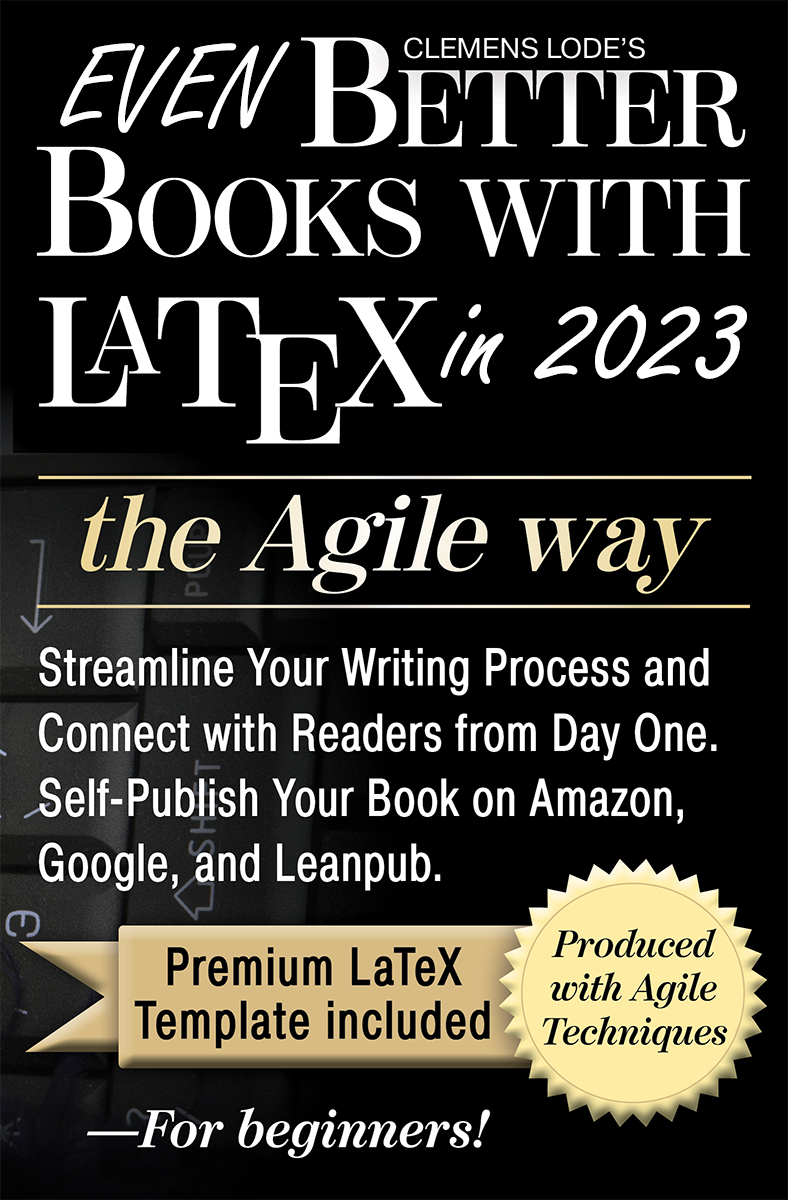
\includegraphics[width=.45\textwidth]{images/cover.jpg}
\end{center}

At LODE Publishing, we also publish works on science, philosophy, and project management. Check out \url{https://www.lode.de/publications} for a list. If you are interested in working with us to publish your book or if you are seeking advice on the next steps to take, contact us at \textbf{mail@lode.de}.

% %%%%%%%%%%%%%%%%%%%%%%%%%%%%%%%%%%%%%
% Check out the accompanying book, Even Better Books with LaTeX the Agile Way in 2023, for a discussion of the template and step-by-step instructions. https://amzn.to/3HqwgXM https://leanpub.com/eBBwLtAW/
% The template was originally created by Clemens Lode, LODE Publishing (www.lode.de), on 1/1/2023. Feel free to use this template for your book project!
% I would be happy if you included a short mention in your book in order to help others to create their own books, too ("Book template based on \textit{Even Better Books with LaTeX the Agile Way in 2023} by Clemens Lode").
% Contact me at mail@lode.de if you need help with the template or are interested in our editing and publishing services.
% And don't forget to follow us on Instagram! https://www.instagram.com/lodepublishing/ https://www.instagram.com/betterbookswithlatex/
%%%%%%%%%%%%%%%%%%%%%%%%%%%%%%%%%%%%%

% This file prints the author page.

% Upload a high-resolution (author_highres.png) and a low-resolution picture (author.jpg) of the author into the images folder and uncomment the 5 includegraphics lines.
% Replace the paragraph about quotations with a quotation of your choice.
% Add text describing your motivation, your professional background, what you are currently doing, and how to connect with you.

\chapter{The Author \yourName}
\label{the-author:cha}

\begin{center}

\ifuseAuthorImage
\ifxetex
	\includegraphics[width=.7\textwidth]{\authorImageHiRes}
\else
	\includegraphics{\authorImage}
\fi
\fi

\end{center}

\begin{myquotation} Here is space for a quotation that describes your journey through life (as opposed to just during the writing of this book). Pick one that best describes you, your attitude, or something you admire. Be personal!\end{myquotation}


Describe your dreams, what goals you have in life, where you went to school or studied, and what job you currently work or worked in the past. Make clear what motivated you to start writing. Finally, add contact points where people can connect with you (mail, Facebook, Instagram, TikTok, YouTube, Twitter, etc.).

% %%%%%%%%%%%%%%%%%%%%%%%%%%%%%%%%%%%%% 
% Check out the accompanying book, Even Better Books with LaTeX the Agile Way in 2023, for a discussion of the template and step-by-step instructions. https://amzn.to/3HqwgXM https://leanpub.com/eBBwLtAW/
% The template was originally created by Clemens Lode, LODE Publishing (www.lode.de), on 1/1/2023. Feel free to use this template for your book project! 
% I would be happy if you included a short mention in your book in order to help others to create their own books, too ("Book template based on \textit{Even Better Books with LaTeX the Agile Way in 2023} by Clemens Lode").
% Contact me at mail@lode.de if you need help with the template or are interested in our editing and publishing services.
% And don't forget to follow us on Instagram! https://www.instagram.com/lodepublishing/ https://www.instagram.com/betterbookswithlatex/
%%%%%%%%%%%%%%%%%%%%%%%%%%%%%%%%%%%%%

% Use this chapter to summarize what you have learned while writing the book. This helps you to write better books in the future, and it might be interesting for the reader to learn how the book came about.

\chapter{The Book's Story}\label{booksstory:cha}

% Add a quotation that encompasses or describes the lessons you learned while planning and writing the book.




% %%%%%%%%%%%%%%%%%%%%%%%%%%%%%%%%%%%%% 
% Check out the accompanying book, Even Better Books with LaTeX the Agile Way in 2023, for a discussion of the template and step-by-step instructions. https://amzn.to/3HqwgXM https://leanpub.com/eBBwLtAW/
% The template was originally created by Clemens Lode, LODE Publishing (www.lode.de), on 1/1/2023. Feel free to use this template for your book project! 
% I would be happy if you included a short mention in your book in order to help others to create their own books, too ("Book template based on \textit{Even Better Books with LaTeX the Agile Way in 2023} by Clemens Lode").
% Contact me at mail@lode.de if you need help with the template or are interested in our editing and publishing services.
% And don't forget to follow us on Instagram! https://www.instagram.com/lodepublishing/ https://www.instagram.com/betterbookswithlatex/
%%%%%%%%%%%%%%%%%%%%%%%%%%%%%%%%%%%%%

\chapter{Reflection}

\begin{problem}
Introductory text about what this section is about. For example, describe that this is a summary of all the ``problem boxes'' throughout the book and point to an online forum where readers can discuss them.\end{problem}

% If you would like to reset formatting, use this code.
\setlength{\parindent}{0.0cm}
\renewcommand{\index}[1]{}
\renewenvironment{problem}[1][]{$\bullet$\ #1}
\footnotesize 


\section*{Replace with Your First Chapter}
% Add questions encountered in your first chapter.
\begin{problem}What is LaTeX?\end{problem}


\section*{Replace with Your Second Chapter}
% Add questions encountered in your second chapter.

\section*{Replace with Your Third Chapter}
% Add questions encountered in your third chapter.
% \index{XeLaTeX@\textit{XeLaTeX}|textbf}
% %%%%%%%%%%%%%%%%%%%%%%%%%%%%%%%%%%%%% 
% Check out the accompanying book, Even Better Books with LaTeX the Agile Way in 2023, for a discussion of the template and step-by-step instructions. https://amzn.to/3HqwgXM https://leanpub.com/eBBwLtAW/
% The template was originally created by Clemens Lode, LODE Publishing (www.lode.de), on 1/1/2023. Feel free to use this template for your book project! 
% I would be happy if you included a short mention in your book in order to help others to create their own books, too ("Book template based on \textit{Even Better Books with LaTeX the Agile Way in 2023} by Clemens Lode").
% Contact me at mail@lode.de if you need help with the template or are interested in our editing and publishing services.
% And don't forget to follow us on Instagram! https://www.instagram.com/lodepublishing/ https://www.instagram.com/betterbookswithlatex/
%%%%%%%%%%%%%%%%%%%%%%%%%%%%%%%%%%%%%

% This file summarizes the conclusions or summaries of each chapter.

\chapter{Eureka!}

\begin{idea}
Introductory text about what this section is about. For example, describe that this is a summary of all the idea boxes throughout the book.\end{idea}

% Use the following command to reformat idea boxes.
\renewenvironment{idea}[1][]{$\bullet$\ #1}

% Use the following command to deactivate the indexing of idea boxes in order to prevent duplicates.
\ifxetex
        \renewcommand{\index}[1]{\ignorespaces}
\fi

\section*{Replace with Your First Chapter}
% Here, you can add ideas presented in your first chapter.
\begin{idea}
LaTeX is a document preparation system.
\end{idea}

\section*{Replace with Your Second Chapter}
% Here, you can add ideas presented in your second chapter.

\section*{Replace with Your Third Chapter}
% Here, you can add ideas presented in your third chapter.
% \index{XeLaTeX@\textit{XeLaTeX}|textbf}
% %%%%%%%%%%%%%%%%%%%%%%%%%%%%%%%%%%%%%
% Check out the accompanying book, Even Better Books with LaTeX the Agile Way in 2023, for a discussion of the template and step-by-step instructions. https://amzn.to/3HqwgXM https://leanpub.com/eBBwLtAW/
% The template was originally created by Clemens Lode, LODE Publishing (www.lode.de), on 1/1/2023. Feel free to use this template for your book project!
% I would be happy if you included a short mention in your book in order to help others to create their own books, too ("Book template based on \textit{Even Better Books with LaTeX the Agile Way in 2023} by Clemens Lode").
% Contact me at mail@lode.de if you need help with the template or are interested in our editing and publishing services.
% And don't forget to follow us on Instagram! https://www.instagram.com/lodepublishing/ https://www.instagram.com/betterbookswithlatex/
%%%%%%%%%%%%%%%%%%%%%%%%%%%%%%%%%%%%%

% This file lists the glossary items throughout the book.

% If you have added or removed any entries in the glossary directory, add them here. If a letter is missing, add a new \section*{} with the letter.

\chapter{Glossary}
\label{glossary:cha}

\section*{C}
\begin{multicols}{2}
\babelEN{\begin{definition}{Citavi} \textit{Citavi} is a plugin for Word (see \url{https://www.citavi.com}) to manage your bibliography and citations.\end{definition}}\index{Citavi@\textit{Citavi}|textbf}
\end{multicols}

\section*{L}
\begin{multicols}{2}
\begin{definition}{LaTeX}\index{latex|textbf} LaTeX is a document preparation system.\end{definition}
\end{multicols}

\section*{O}
\begin{multicols}{2}
\babelEN{\begin{definition}{Overleaf} \textit{Overleaf} is an online editor and project manager for LaTeX documents. It manages your project with a versioning system and automatically compiles your LaTeX code into PDF and (with some help) HTML. It is free for public projects and does not require installation or setup. You can get an account here: \url{https://www.overleaf.com}.\end{definition}}\index{Overleaf@\textit{Overleaf}|textbf}

\end{multicols}

\section*{P}
\begin{multicols}{2}
\begin{definition}{pdfLaTeX} \textit{pdfLaTeX} is a basic LaTeX typesetting engine that translates LaTeX documents directly into PDFs or HTML files (with the help of \textit{TeX4ht}).\end{definition}\index{pdfLaTeX@\textit{pdfLaTeX}|textbf}
\end{multicols}

\section*{V}
\begin{multicols}{2}
\begin{definition}{Versioning system} A \textit{versioning system} is a tool to track changes to a document. That means you can go back and check what has been changed and by whom.\end{definition}\index{versioning system|textbf}
\end{multicols}

\section*{W}
\begin{multicols}{2}
\begin{definition}{Word} \textit{Word} usually refers to \textit{Microsoft Word}. Generally, it is used as an umbrella term for all word processors that directly show you what you will get as an end result (as opposed to first having to process the file). This approach is intuitive, but it makes editing large projects very complicated.\end{definition}\index{Word@\textit{Word}|textbf}
\end{multicols}

\section*{X}
\begin{multicols}{2}
\begin{definition}{XeLaTeX} \textit{XeLaTeX} is a LaTeX typesetting engine with an extended font, as well as UTF-8 encoding (for special characters) support. It takes longer to compile with \textit{XeLaTeX} than with the more basic \textit{pdfLaTeX}.\end{definition}\index{XeLaTeX@\textit{XeLaTeX}|textbf}




\end{multicols}


% This adds a separate quotations page (sources in the e-book are already included in the text body).
% \ifxetex
%     %%%%%%%%%%%%%%%%%%%%%%%%%%%%%%%%%%%%%
% Check out the accompanying book, Even Better Books with LaTeX the Agile Way in 2023, for a discussion of the template and step-by-step instructions. https://amzn.to/3HqwgXM https://leanpub.com/eBBwLtAW/
% The template was originally created by Clemens Lode, LODE Publishing (www.lode.de), on 1/1/2023. Feel free to use this template for your book project!
% I would be happy if you included a short mention in your book in order to help others to create their own books, too ("Book template based on \textit{Even Better Books with LaTeX the Agile Way in 2023} by Clemens Lode").
% Contact me at mail@lode.de if you need help with the template or are interested in our editing and publishing services.
% And don't forget to follow us on Instagram! https://www.instagram.com/lodepublishing/ https://www.instagram.com/betterbookswithlatex/
%%%%%%%%%%%%%%%%%%%%%%%%%%%%%%%%%%%%%

% This file adds a page with quotation sources you have used in your book.

% This is displayed only for print PDFs where the source is not directly mentioned in the text body.

\chapter{Quotation Sources}

\setlength{\parindent}{0pt}
\footnotesize

\babelES{\textbf{\pageref{gogh-sky-quote}:} \cite[vgl.][S.~23--24]{ifyouwanttowrite}}
\babelEN{\textbf{\pageref{gogh-sky-quote}:} \cite[pp.~23--24]{ifyouwanttowrite}}\par

% \fi

% %%%%%%%%%%%%%%%%%%%%%%%%%%%%%%%%%%%%%
% Check out the accompanying book, Even Better Books with LaTeX the Agile Way in 2023, for a discussion of the template and step-by-step instructions. https://amzn.to/3HqwgXM https://leanpub.com/eBBwLtAW/
% The template was originally created by Clemens Lode, LODE Publishing (www.lode.de), on 1/1/2023. Feel free to use this template for your book project!
% I would be happy if you included a short mention in your book in order to help others to create their own books, too ("Book template based on \textit{Even Better Books with LaTeX the Agile Way in 2023} by Clemens Lode").
% Contact me at mail@lode.de if you need help with the template or are interested in our editing and publishing services.
% And don't forget to follow us on Instagram! https://www.instagram.com/lodepublishing/ https://www.instagram.com/betterbookswithlatex/
%%%%%%%%%%%%%%%%%%%%%%%%%%%%%%%%%%%%%

% This file prints the bibliography.

%  Uncomment the command below if you want to add a preface to the bibliography (between the title and the list of referenced books). See https://tex.stackexchange.com/questions/197061/text-between-index-or-bibliography-title-and-content

%\bibpreface {Add the preface of your list of recommended reading titles here. Delete this line to have no preface for this section.}

\ifxetex
    \printbibliography
\else
    \bibliographystyle{plainnat}
    \babelEN{\bibliography{chapters/bibliography/english}}
\fi


%%%%%%%%%%%%%%%%%
% Appendix
%%%%%%%%%%%%%%%%%
% \appendix

% The index page exists only for printed PDFs.
\ifxetex
    % This is an optional command to display a prologue before the index.
    % \indexprologue{Replace index prologue with an own introduction (errata, formatting, abbreviations, etc.).}

    \printindex
    \thispagestyle{empty}
\fi

% %%%%%%%%%%%%%%%%%%%%%%%%%%%%%%%%%%%%% 
% Check out the accompanying book, Even Better Books with LaTeX the Agile Way in 2023, for a discussion of the template and step-by-step instructions. https://amzn.to/3HqwgXM https://leanpub.com/eBBwLtAW/
% The template was originally created by Clemens Lode, LODE Publishing (www.lode.de), on 1/1/2023. Feel free to use this template for your book project! 
% I would be happy if you included a short mention in your book in order to help others to create their own books, too ("Book template based on \textit{Even Better Books with LaTeX the Agile Way in 2023} by Clemens Lode").
% Contact me at mail@lode.de if you need help with the template or are interested in our editing and publishing services.
% And don't forget to follow us on Instagram! https://www.instagram.com/lodepublishing/ https://www.instagram.com/betterbookswithlatex/
%%%%%%%%%%%%%%%%%%%%%%%%%%%%%%%%%%%%%

% This file adds a page reminding the reader to leave a review.

% Replace this with your own call to action or use the default text.
\chapter{An Important Final Note}

% Show this paragraph only for e-books.
\ifxetex \else \textit{If you want to rate this e-book, please also add a short text comment. Without a text comment, your star rating will be invisible on the Amazon website and count only as an indicator for additional recommendations on Amazon. Thanks!}\fi

% Show the following for e-books and printed books. 
Writers are not performance artists. While there are book signings and public readings, most writers (and readers) follow their passion alone in their homes.

\textit{What applause is for the musician, \textbf{reviews} are for the writer.} 

\textit{Books create a community among readers}; you can share your thoughts among all those who will or have read the book.

\textbf{Leave a thoughtful, honest review and help me to create such a community on the platform on which you have acquired this book.} 
\textit{What did you like, what can be improved? To whom would you recommend it?} 

Thank you, also in the name of all the other readers who will be able to better decide whether this book is right for them or not. A positive review will increase the reach of the book; a negative review will improve the quality of the next book. I welcome both!
% %%%%%%%%%%%%%%%%%%%%%%%%%%%%%%%%%%%%% 
% Check out the accompanying book, Even Better Books with LaTeX the Agile Way in 2023, for a discussion of the template and step-by-step instructions. https://amzn.to/3HqwgXM https://leanpub.com/eBBwLtAW/
% The template was originally created by Clemens Lode, LODE Publishing (www.lode.de), on 1/1/2023. Feel free to use this template for your book project! 
% I would be happy if you included a short mention in your book in order to help others to create their own books, too ("Book template based on \textit{Even Better Books with LaTeX the Agile Way in 2023} by Clemens Lode").
% Contact me at mail@lode.de if you need help with the template or are interested in our editing and publishing services.
% And don't forget to follow us on Instagram! https://www.instagram.com/lodepublishing/ https://www.instagram.com/betterbookswithlatex/
%%%%%%%%%%%%%%%%%%%%%%%%%%%%%%%%%%%%%
% This file is the last page of the book.

\thispagestyle{empty}
\ifxetex
    \vspace*{\fill}
\fi
\hfill

% Replace the quote.
\babelEN{\begin{myquotation} Replace this quote\par\mbox{}\hfill \emdash{}Name of the author\end{myquotation}}

\end{document}
